\documentclass[twocolumn,a4paper,10pt]{article}

\usepackage[utf8]{inputenc}
\usepackage[english]{babel}
\usepackage[T1]{fontenc}
%%%%%% MISE EN PAGES %%%%%%
\usepackage[width=175mm, top=3cm]{geometry}

\setcounter{tocdepth}{3}     % Dans la table des matieres
\setcounter{secnumdepth}{4}  % Avec un numero.

% \renewcommand{\chaptermark}[1]{\markboth{\thechapter.\space#1}{}} 
\usepackage{layout}

%%%%%% SYMBOLES %%%%%
\usepackage{tipa}	% pour avoir l'accent concave
\usepackage{lmodern}	% pour les guillemets
\usepackage{nth}

%%%%%% EQUATION %%%%%%
\usepackage{amssymb}
\usepackage{amsmath}
\usepackage{fancybox}
\usepackage{xfrac}	% fraction de type "1/4"
\usepackage{cases}	% système équation
\usepackage[overload]{empheq}
\usepackage{bm}		% pour mettre en gras .
\usepackage{units} 	% x/y barre latérale pour les fractions

%%%%%% FIGURE %%%%%%
\usepackage{graphicx}	% insérer des graphiques
\usepackage{subfigure}	% utiliser subfigure
\usepackage{float}	% utiliser H dans les figures

%%%%%% TABLEAUX %%%%%%
\usepackage{array,multirow,makecell}
%\addto\captionsfrench{\def\tablename{\textsc{Tableau}}}% pour avoir TABLEAU et pas TABLE dans les légendes des tableaux
\usepackage[table,xcdraw]{xcolor} % pour avoir des lignes colorées dans les tableau
\usepackage{slashbox} % pour les \backslashbox
%\usepackage{subcaption}
\usepackage{hhline}	% pour les lignes horizontales 
\usepackage{tabularx} % permet itemize dans les cellules


\newcolumntype{L}[1]{>{\raggedright\let\newline\\\arraybackslash\hspace{0pt}}m{#1}}
\newcolumntype{C}[1]{>{\centering\let\newline\\\arraybackslash\hspace{0pt}}m{#1}}
\newcolumntype{R}[1]{>{\raggedleft\let\newline\\\arraybackslash\hspace{0pt}}m{#1}}

%%%%%%%%%%%%%%%%%%%%%
\usepackage{url}	% gérer les adresses www.
\linespread{1}	% interligne

\cleardoublepage

\newcommand{\ml}[1]{\textcolor{blue}{ Mathieu: #1}}

\title{Estimation of the road traffic sound levels in urban areas based on non-negative matrix factorization techniques}

\author{
    Jean-Rémy GLOAGUEN\\
    Arnaud Can\\
    LAE\\
    Ifsttar\\
    jean-remy.gloaguen@ifsttar.fr
  \and
    Mathieu Lagrange\\
	Jean-François Petiot \\
    LS2N, CNRS\\
    \'Ecole Centrale de  Nantes\\
}
\date{}
\begin{document}

\maketitle

\section*{Abstract}

The advent of low cost acoustic monitoring devices raises new interesting approaches for improving the monitoring the acoustic quality of urban areas. Assuming that transportation is the major source of annoyance, state of the art approaches consider as input an estimate of the number and the speed of vehicules in major traffic lanes. Follows a prediction procedure that outputs an acoustic pressure level at any location in the modeled area.

Considering as input the acoustic pressure measured in many locations using a sensor grid approach would greatly complement and improve the quality of the predicted pressure values. Among the technical issues that raises this kind of innovative approaches, there is a need to identify which part of the overall acoustic pressure level is due to the road traffic.

In this paper, several techniques based on the non-negative factorization framework are studied in this application scenario. The task being to the best of our knowledge never been considered in the literature, we propose an exprimental protocol to validate the studied approaches that complies with standard reproducible research recommandations.

\section{Introduction}

With the introduction of the European Directive 2002/EC/49, cities over 100 000 inhabitants have to produce road traffic noise maps. These maps depict an estimation of the number of city dwellers exposed to high noise levels. They are used to draw up action plans to reduce it as too long exposures to these noises can generate health problems \cite{who_burden_2017}. These maps are the result of a simulation process based on the estimation of the traffic density on the main roads and the use of sound propagation techniques. They express $L_ {DEN}$ and $L_N$, which are \textit{Day-Evening-Night} and \textit{Night} equivalent A-weighted sound levels respectively. However, these maps introduce lot of uncertainty generated by the numerical tools \cite{van_leeuwen_noise_2015}, by the different calculation methodologies used \cite{leroy_uncertainty_2010}\cite{garg_critical_2014} \ml{un peu hors propos on améliore rien la dessus : or even by the calculation procedure of the number of inhabitants exposed to noise \cite{king_implementation_2011}. plutot parler du cote sparse des données d'entrées}. In addition, the usual road traffic noise maps are static, aggregating the exposure on the two indicators $L_{DEN}$ and $L_N$, thus ignoring the sound levels evolution throughout the day. Since the creation of road traffic noise maps entails long data collection and calculation times, the use of acoustic measurements could facilitate their updating or even the generation of dynamic maps \cite{wei_dynamic_2016}. These measurements can be performed at fixed stations spread all over the cities \cite{Mioduszewski} \cite{mietlicki2012innovative}, which would lead to the availability of the long-term evolution of the traffic noise levels. It can also be performed with  mobile stations \cite{can_exploring_2012} \cite{manvell2004sadmam} covering a larger area with fewer sensors but also sparse time periods.

Currently, sensor networks in cities are spread for multiple applications (air quality assessment, measurement of meteorological parameters ...), including the assessment of urban noise levels. DYNAMAP project \cite{dynamap_2016} studied the deployment and feasibility of such installations. It focuses on sensor installations on specific roads at the city scale in Milan and Rome \cite{bellucci_life_2017}. In a similar way, but reduced to few neighborhoods \ml{with a more dense topology ? parler aussi de sonyc}, the CENSE project\footnote{\url{http://cense.ifsttar.fr/}} \cite{picaut2017characterization} aims to combine \textit{in situ} observations, from a sensor network, and numerical data, from noise modeling, through data assimilation techniques.

If sensor networks could improve road traffic noise estimates compared with simulated maps, the issue of the correct estimation of the traffic sound level from acoustic measurements is still unsolved \cite{Mioduszewski}. Indeed, the urban sound environment is a complex environment gathering lots of different sounds (car passages, voices, whistling bird, car horn, airplanes \dots) that overlap. Consequently, the traffic sound level estimation based on measurements is not a trivial task.
Many recent works have focused on the detection or recognition tasks of environmental sounds \cite{heittola_sound_2011}, \cite{defreville_automatic_2006}, \cite{dufaux_automatic_2000}, \cite{chu_environmental_2009}. A two-step process is generally followed : describe the audio files with a set of features (Spectrum Gravity Spectrum, harmonicity, Mel-Frequency Cepstral Coefficient \dots) and classify them with the help of classifiers (Support Vector Machines, Gaussian Mixture Models, Hidden Markov Model, Artifical Neural Networks). A description of these features and classifiers can be found in \cite{cowling_comparison_2003} and their applications can be found in \cite{shen_environmental_2012}, \cite{beritelli_pattern_2008}, \cite{couvreur_automatic_2004}.

The main issue in the detection or recognition tasks is the overlap of environmental sounds. Although near major roads or ring roads, traffic is predominant, there are many places where it overlaps with other sound sources that contribute significantly to the overall sound levels. To circumvent this issue, Socoro et al. propose to suppress time frames where there is significant overlap by considering an Anomalous Noise Events Detector \cite{socoro_anomalous_2017} which consist in detecting the unwanted sound sources from labeled recordings, \textit{i.e.} that are not related to the traffic component. Those time frames are then discarded in order not to take them into account during the estimation of the traffic sound level.  \ml{arrete :) If the detection of the road traffic noise is good, the detection of these anomalous noise events stay a complicated task \cite{stowell2015detection}.}

An alternative approach that we will foolow in this paper is to consider the blind source separation paradigm to reliably estimate the traffic noise level. That is, separating the contribution of the traffic from the other sources within a polyphonic scene. One major advantage of following such approach is that the estimate is continuously available, making the approach applicable in a wide range of urban areas, even where the traffic noise is relatively low compared to the remaining contributions.\\

ml{Supprimer : One of the first to do so is the Independent Component Analysis \cite{comon_independent_1994}. The principle is to decompose $N$ recorded signals to a sum of $P$ independent sound sources weighted by linear relations. This method is most of all suited for the 'cocktail party' issue where one tries to capture a signal among noise. In an urban environment context, this method is used with acoustic microphone arrays and beamforming \cite{saruwatari2003blind}. These approaches consider a set of microphones and allows the localization \cite{mennitt2010multiple} or the detection \cite{leiba2017large} of sound sources from the phase shift and the distance between the microphones. However, one need a lot of microphones. Spread multiples microphones arrays in cities is then expensive (even with low cost microphones) and is time-consuming for calibration and maintenance.}

A convenient method for monophonic signal decomposition is the Non-negative Matrix Factorization (NMF) technique \cite{lee_learning_1999}. When considering audio as input, it usually consists in approximating the magnitude spectrogram of an audio file by the product of two low rank matrices, one representing the components of interest and the other the contribution at a given time of those components to approximate the input magnitude spectrogram \cite{smaragdis_non-negative_2003} \cite{wilson_speech_2008} \cite{mesaros_sound_2015}. In the audio processing domain, the NMF has already been employed for the source separation task of monaural signals of speech and music \cite{wang_musical_2005} \cite{wilson_speech_2008}. By design, this method deals reasonably well with the overlaping sound sources as soon as the overlap can be resolved on the time/frequency plane. \ml{enlever : For the environmental sounds, the method has been used for the geo-localisation and classification of the sound environment, like in \cite{kumar_audio_2016} where NMF is used to classify the audio files according to the 10 cities where they have been recorded.}

Closer to our application scenario, NMF has been considered by Innami and Kasai \cite{satoshi_innami_nmf-based_2012}. After having performed NMF on simulated audio files, they perform a source separation based on NMF in two steps by 1) separating the sound background from the events and 2) by isolating the events using spectral features using a $k$-means procedure.



\ml{ enlever : A $k$-mean clustering allows the separation of the $k$ sound sources. This approach, compared to a simple MFCC clustering, improves the sound source separation but the authors admit their approach need the assumption that the number of sound sources is known which is unrealistic in practical case.  Furthermore, in order to estimate the traffic sound level $\tilde{L}_{p,traffic}$, their approach might be difficult to be adapted it as traffic component can be both sound background and event.}

We study in this paper different flavors of Non-Negative Matrix Factorization (NMF) where traffic component is considered in its entirely whether it is a sound background or event. We demonstrate the supervised NMF and semi supervised NMF approaches have some interests but fail to give satifactory results for the application at hand. We thus introduce another NMF scheme called thresholded initialized NMF that make good use of prior knowledge about the source of interest, in our case the traffic noise, but also generalizes well to several kinds of urban areas and to traffic to interference ratio (TIR).

To perform the numerical experiments, we consider a corpus of simulated sound scenes created from a built-up sound database composed of a high number of diverse sound samples. The use of simulated sound scenes is mandatory for rigorous experimental validation as it offers a high level of control on the design of the scenes and the knowledge of the exact contribution of the traffic component ($L_{p,traffic}$) which would be difficult to extract from a recording of an urban scene.

\begin{figure*}[t]
\centering
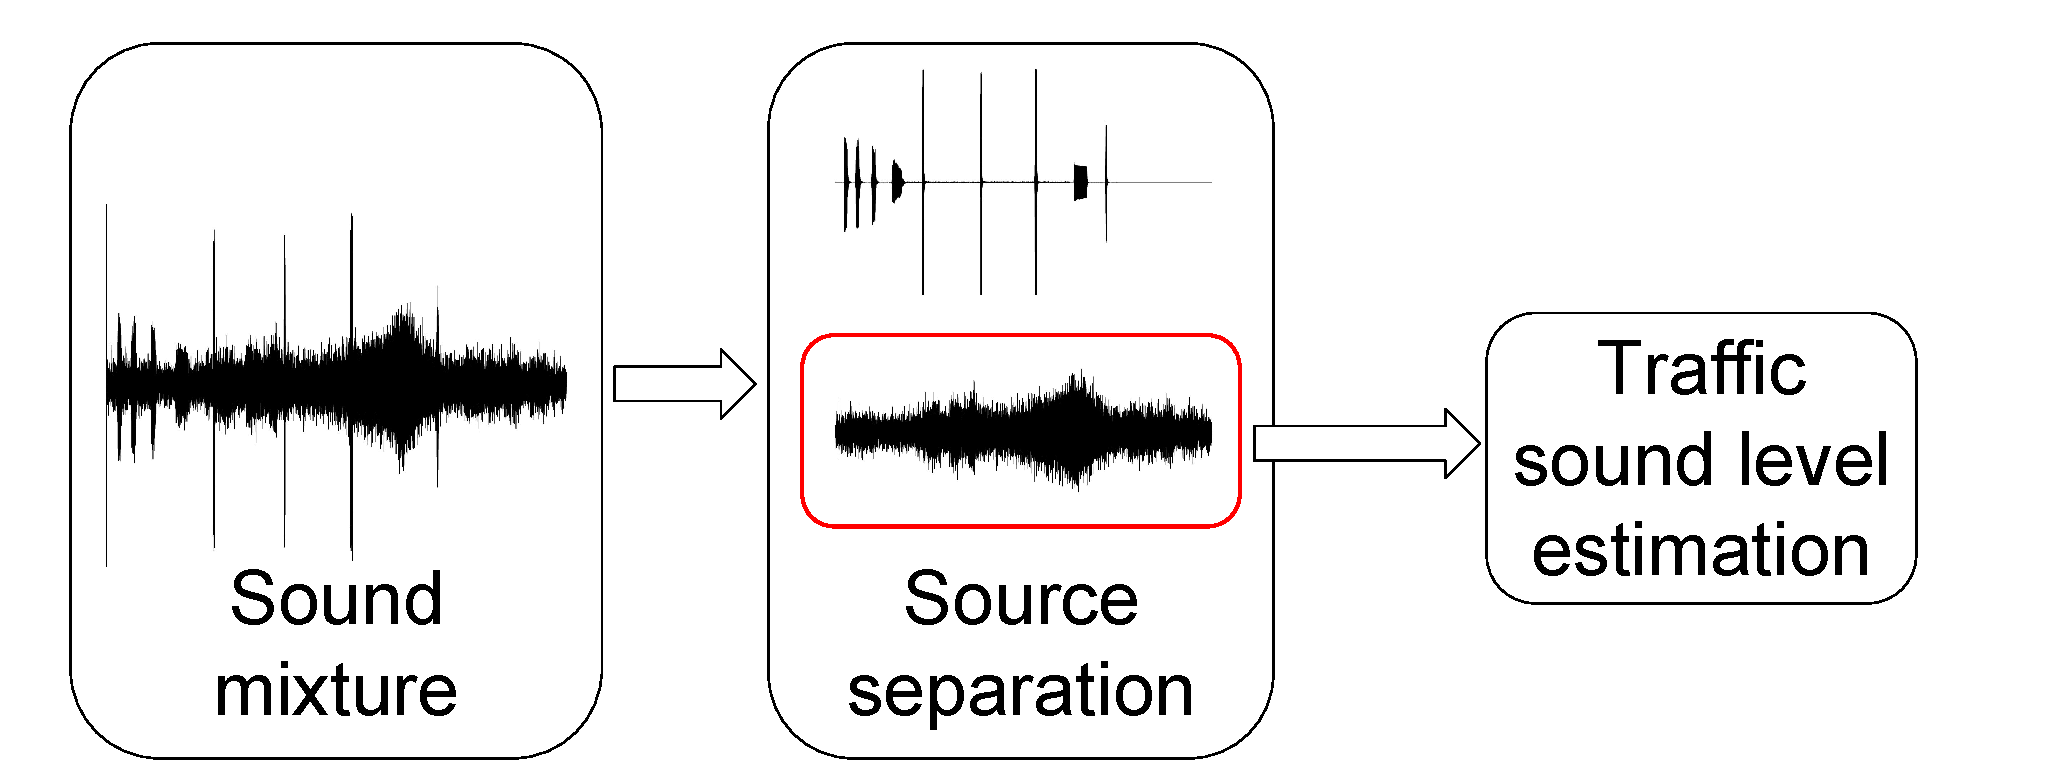
\includegraphics[width=0.7\textwidth]{figures/bloc_diagram_source_separation.pdf}
\caption{Block diagram of the source separation method. \ml{toujours citer une figure}}
\label{fig:diagram}
\end{figure*}

The remaining of the paper is organized as follows. Section \ref{part:nmf} details the technical aspects of NMF and describes the 3 approaches considered in this paper to achieve the task at hand. Section \ref{part:protocol} describes the environmental sound scene corpus and the experimental protocol setup. Section \ref{part:results} then describes and discusses the outcomes of the numerical experiments.

\section{Non-negative Matrix Factorization}\label{part:nmf}
\subsection{Description of NMF}

Non-negative Matrix Factorization is a linear approximation method introduced by Lee and Seung, \cite{lee_learning_1999}, which can be used to approximate the spectrogram (obtained using a Short-Term Fourier Transform) of an audio file, $\mathbf{V}$, $\in \mathbb{R}^+_{F \times N}$ as :

\begin{equation}\label{eq:nmf}
\mathbf{V} \approx \mathbf{\tilde{V}} = \mathbf{WH}
\end{equation}

where $\mathbf{W} \in \mathbb{R}^+_{F \times K}$ is the \textit{dictionary} (or basis) matrix composed of audio spectrum and $\mathbf{H} \in \mathbb{R}^+_{K \times N}$ is the \textit{activation} matrix which summarizes the temporal evolution of each element of $\mathbf{W}$. An illustrative example can be found in Figure  \ref{fig:example_NMF}.

\begin{figure}[t]
\centering
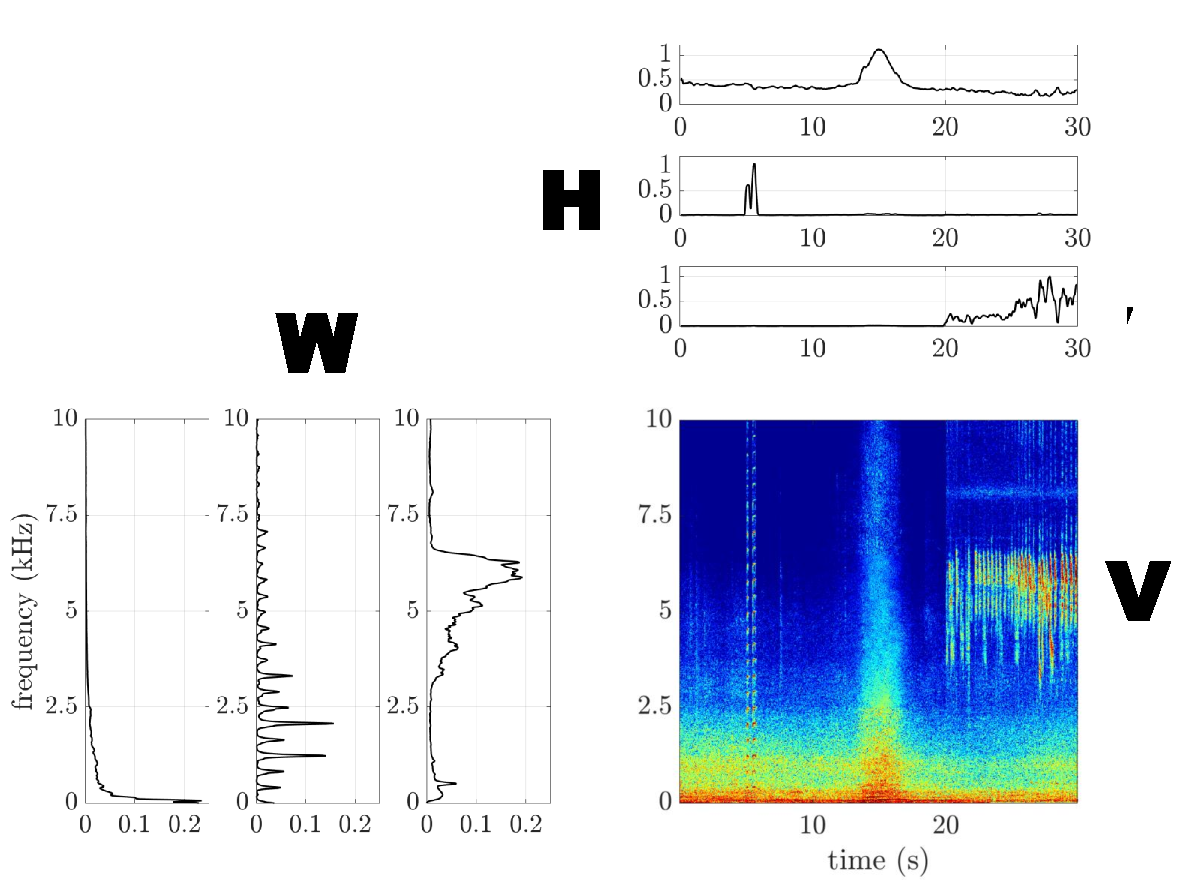
\includegraphics[width=0.9\linewidth]{figures/schema_introduction_nmf.pdf}
\caption{Example of a simple NMF  for urban sound mixture, $\mathbf{W}$ and $\mathbf{V}$ are composed of 3 elements (car passages, car horn and bird's whitles)}
\label{fig:example_NMF}
\end{figure}

The choice of the dimensions is often made as that $F\times K + K \times N < F \times N$. NMF is then considered as a low rank approximation method. However, this constraint is not mandatory. To estimate the quality of the approximation, an objective function is used

\begin{equation}\label{eq:min-D-WH}
\underset{\mathbf{H} \geq 0, \mathbf{W} \geq 0}{\min} D\left(\mathbf{V} \vert \vert \mathbf{\tilde{V}}\right).
\end{equation}

The operator $D(x\vert y)$ is a divergence calculation such as:
\begin{equation}
D\left(\textbf{V} \vert\vert \mathbf{\tilde{V}} \right) = \sum_{f = 1}^{F} \sum_{n = 1}^{N} d_{\beta}
\left(\textbf{V}_{fn} \vert \left[ \textbf{WH} \right]_{fn} \right)
\end{equation}

and usually belongs to the $\beta-$divergence class \cite{fevotte_nonnegative_2009} in which the well known Euclidean distance (eq. \ref{eq:def_distEUC}) and the Kullback-Leibler divergence (eq. \ref{eq:def_divKL}) belong

\begin{subequations}\label{eq:divBetaGenerale}
\begin{numcases}{d_{\beta}(x\vert y) =}
    \frac{1}{2}(x-y)^2, & $\beta = 2$, \label{eq:def_distEUC}\\
    x\log \dfrac{x}{y} - x + y, & $\beta = 1$.\label{eq:def_divKL}
\end{numcases}
\end{subequations}

To better take account prior knowledge on the sources,  constraints (like the smoothness or the sparsness criteria \cite{virtanen_monaural_2007}) can be added to the objective function.

Algorithms have been proposed to solve the minimization problem (\ref{eq:min-D-WH}) iteratively such as the multiplicative update \cite{lee_algorithms_2000}, the alternating least square method \cite{cichocki_regularized_2007}, the projected gradient \cite{lin_projected_2007} \dots Here, the multiplicative update is chosen as it ensures non-negative results of which convergence has been proved \cite{fevotte_algorithms_2011}.

\subsection{Supervised NMF}
First, supervised NMF (SUP NMF) is used: the \textit{dictionary} includes audio spectrum of urban sound sources. In the urban environments, a lot of different sound sources present are known whose spectrum can be obtained and be a basis of $\mathbf{W}$. The \textit{activator} are then the unknown to estimate. In the first iteration, $\mathbf{H}$ is initialized randomly, then it is updated by the generic algorithm

\begin{equation}\label{eq:updateH_Sup}
\textbf{H}^{(i+1)} \leftarrow \textbf{H}^{(i)}.\left(\frac{\textbf{W}^T \left[\left(\textbf{WH}^{(i)} \right)^{(\beta-2)}.\textbf{V} \right]}{\textbf{W}^T \left[\textbf{WH}^{(i)} \right]^{(\beta-1)}}\right)^{\gamma(\beta)}
\end{equation}

with $\gamma(\beta) = \frac{1}{2-\beta},$ for $\beta < 1$, $ \gamma(\beta) = 1$, for $\beta \in \left[1,2\right]$ and $\gamma(\beta) = \frac{1}{\beta-1}$ for $\beta > 2$. The product $A.B$ and $A/B$ symbolized the Hadamard product and ratio. As in the supervised approach, the position in $\mathbf{W}$ of traffic component is known, the separation of this sound source is made by extracting the related basis and activators,

\begin{equation}\label{eq:separationExtraction}
\mathbf{\tilde{V}}_{traffic} = \left[ \mathbf{WH} \right]_{traffic}.
\end{equation}

\subsection{Semi-supervised NMF}

One of the main issue with the supervised approach is the generalization issue: how to be adapted to different sound mixtures with a fixed dictionary ? To better take into account the diverse nature of urban scenes, semi-supervised NMF (S-S NMF)\cite{lee_semi-supervised_2010} can be useful as it has been proposed  to offer more flexibility. This method consists in composing the \textit{dictionary} with a fixed part $\mathbf{W_s} \in \mathbb{R}^+_{F\times K}$, composed in our case of road traffic spectrum, and with a mobile part, $\mathbf{W_r} \in \mathbb{R}^+_{F\times J}$ with $J <<K$, that is updated. Here, $J = 2$. The aim is to include in $\mathbf{W_r}$ the elements that are not related with the traffic. The problem (\ref{eq:nmf}) becomes

\begin{equation}
\mathbf{V} \approx \mathbf{W_s H_s}+ \mathbf{W_r H_r}
\end{equation}

 with $\mathbf{W} = \left[\mathbf{W_s} \mathbf{W_r} \right]$ and $\mathbf{H} = \genfrac[]{0pt}{0}{\mathbf{H_s}}{\mathbf{H_r}}$. In a similar way as to solve the equation (\ref{eq:min-D-WH}), $\mathbf{W_r}$, $\mathbf{H_r}$ and $\mathbf{H_s}$ are successively updated with the relations (\ref{eq:WH-SSupdate}):

{\scriptsize
\begin{subequations}\label{eq:WH-SSupdate}
\begin{align}
\mathbf{W_r}^{(i+1)} &\leftarrow \mathbf{W_r}^{(i)}.\left(\frac{\left[\left(\mathbf{W_r H_r}^{(i)} \right)^{(\beta-2)}.\mathbf{V} \right]\mathbf{H_r}^T}{\left(\mathbf{W_r H_r}^{(i)} \right)^{(\beta-1)}\mathbf{H_r}^T}\right)^{\gamma(\beta)}, \label{eq:W_r_SS}\\
\mathbf{H_r}^{(i+1)} &\leftarrow \mathbf{H_r}^{(i)}.\left(\frac{\mathbf{W_r}^T \left[\left(\mathbf{W_r H_r}^{(i)} \right)^{(\beta-2)}.\mathbf{V} \right]}{\mathbf{W_r}^T \left(\mathbf{W_r H_r}^{(i)} \right)^{(\beta-1)}}\right)^{\gamma(\beta)}, \label{eq:H_r_SS}\\
\mathbf{H_s}^{(i+1)} &\leftarrow \mathbf{H_s}^{(i)}.\left(\frac{\mathbf{W_s}^T \left[\left(\mathbf{W_s H_s}^{(i)} \right)^{(\beta-2)}.\mathbf{V} \right]}{\mathbf{W_s}^T \left(\mathbf{W_s H_s}^{(i)} \right)^{(\beta-1)}}\right)^{\gamma(\beta)}.\label{eq:H_s_SS}
\end{align}
\end{subequations}}

Applications of S-S NMF for speech denoising from background noise or musical content can be found in \cite{joder2012real} and \cite{weninger2012supervised}.

\subsection{Thresholded initialized NMF}

A last approach is tested based on unsupervised NMF. Usually, $\mathbf{W}$ is learnt with the help of a learning corpus by initiated it randomly. Here, as the concerned sound source is known and audio samples of car passages are available, a initial dictionary, $\mathbf{W_0}$, is learnt by converting the audio files in the spectra domain; see part \ref{part:dictionary_learning}. Then NMF is performed where $\mathbf{W}$ (eq. \ref{eq:updateW_unsup}) and $\mathbf{H}$ (eq.  \ref{eq:updateH_Sup}) are updated alternatively. $\mathbf{W}$ is therefore updated by forcing its initiation with \textit{a priori} knowledge.

\begin{equation}\label{eq:updateW_unsup}
\textbf{W}^{(i+1)} \leftarrow \mathbf{W}^{(i)}.\left(\frac{\left[\left(\mathbf{W}^{(i)}\mathbf{H} \right)^{(\beta-2)}.\mathbf{V} \right]\mathbf{H}^T}{\left[\mathbf{W}^{(i)}\mathbf{H} \right]^{(\beta-1)}\mathbf{H}^T}\right)^{\gamma(\beta)}
\end{equation}

After $N$ iterations, a measure of similarity $D_{\theta}\left(\mathbf{W_0} \vert \vert \mathbf{W} \right)$ between $\mathbf{W_0}$ and the get dictionary $\mathbf{W}$ for each element $k$ is computed through a cosine similarity,

\begin{equation}
D_{\theta}\left(\mathbf{W_0} \vert \vert \mathbf{W} \right) = \frac{\mathbf{W}.\mathbf{W_0}}{\vert \vert \mathbf{W}  \vert \vert . \vert \vert \mathbf{W_0} \vert \vert}.
\end{equation}

$D_{\theta}\left(\mathbf{W_0} \vert \vert \mathbf{W} \right) = 1$ means that the elements are identical (the $k$-th element of $\mathbf{W}$ is then considered as traffic element) whereas $D_{\theta}\left(\mathbf{W_0} \vert \vert \mathbf{W} \right)$ = 0 means that the elements are significantly different. This measure is bounded between 1 and 0 and is an invariant scale estimation of the similarity. Then, $D_{\theta}\left(\mathbf{W_0} \vert \vert \mathbf{W} \right)$ is sorted in descending order. The elements in $\mathbf{W}$ that can belong to $\mathbf{W}_{traffic}$ are then selected by a \textit{hard thresholding} method. It is defined as:

\begin{equation}
\mathbf{W}_k \in \mathbf{W}_{k,traffic} \quad \text{iff} \quad D\left(\mathbf{W}_{0,k} \vert \vert \mathbf{W}_{k} \right) > t
\end{equation}

An illustrative example can be see in Figure \ref{fig:W_TI_NMF}.\\

\begin{figure}[hbtp]
\centering
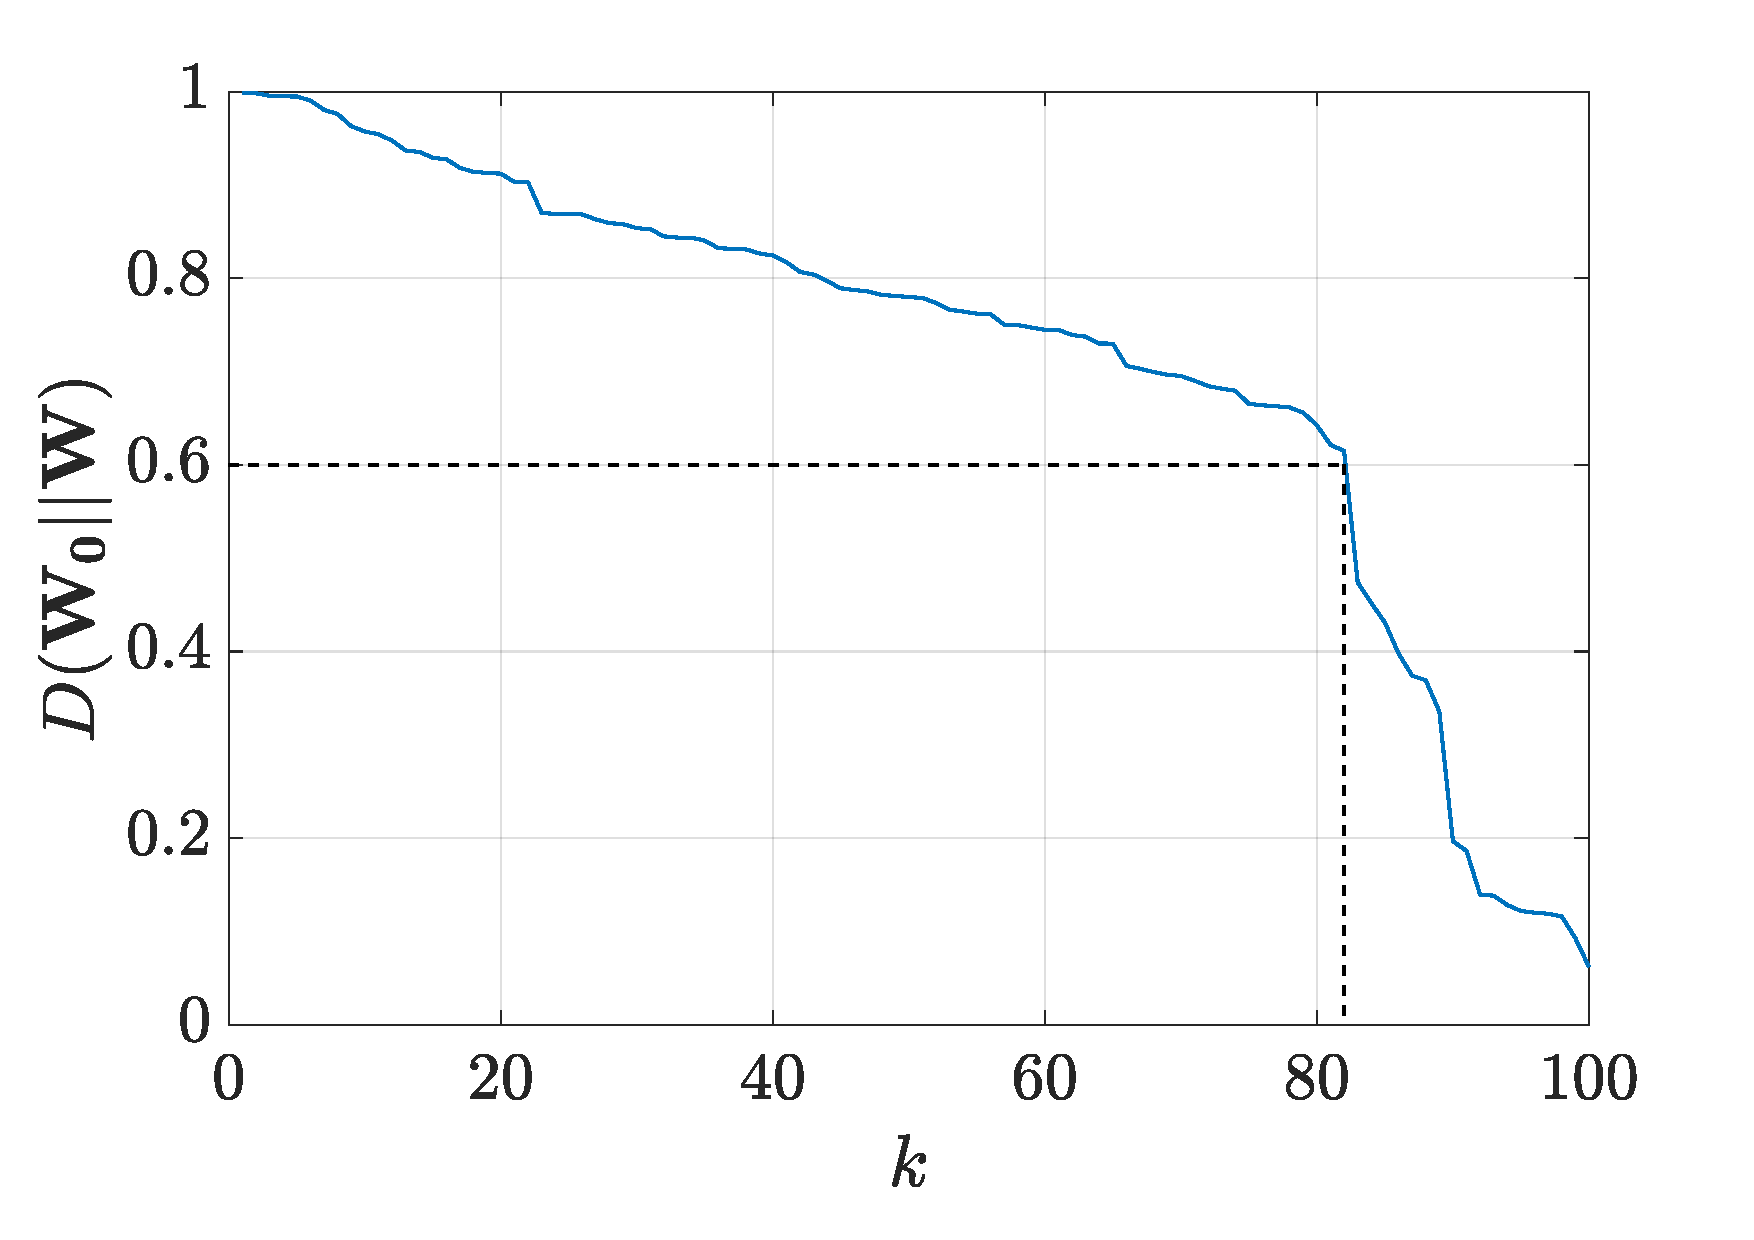
\includegraphics[width=0.8\linewidth]{figures/distanceCosLinDisplay.pdf}
\caption{Example of the $\mathbf{W}_{traffic}$ extraction from the sorted cosine similarity with a threshold $t = 0.6$. The $82$-nd first elements are considered as traffic component.}
\label{fig:W_TI_NMF}
\end{figure}

This approach is named \textit{Thresholded inititialized NMF} (TI NMF). Other thresholding methods as the \textit{soft} \cite{donoho1995noising} and the \textit{firm} \cite{fornasier2008iterative} and multiples way to display the similarity through a sigmoïd or a Radial Basis Function have been investigated. A fast parametric study has revealed that the \textit{hard} thresholding method  with a linear representation of the similarity according to $K$, as in  Figure \ref{fig:W_TI_NMF}, was the best way to get better performances.

\section{Experimental protocol}\label{part:protocol}

In order to validate the usefulness of considering NMF framework to estimate the road traffic noise level, one need to have a reference level. It can hardly be measured or even annotated from real life recordings. Thus,  simulated sound scenes are used to assess the performance of the proposed NMF. This offers a controlled framework to design specific sound environments in which all the traffic component is known. Then, the estimated road traffic sound levels with the method can be compared to the real ones, introduced within each simulated sound scene.

\subsection{Environmental sound scene corpus}

A corpus is designed with the \textit{SimScene} software\footnote{Open-source project available at: \url{https://bitbucket.org/mlagrange/simScene}}. \textit{SimScene} \cite{rossignol_simscene:_2015} is a simulator that creates sound scenes in a .wav format by summing audio samples that come from an isolated sound database.

This database is divided in two categories: $i)$ the \textit{event} category which are the brief sounds (from 1 to 20 seconds) that are considered as salient including 245 sound event samples divided in 19 sound classes (\textit{ringing bell, birds, sweeping broom, car horn, car passages, hammer, drill, coughing, barking dog, rolling suitcase, closing door, plane, siren, footstep, storm, street noise, train, tramway, truck and voice}) and $ii)$ the \textit{background} category that includes all the sounds that are of long duration and whose acoustic properties do not vary with respect to time. 154 sound samples belong to this category divided in 9 sound classes (\textit{birds, construction site noise, crowd, park, rain, children playing in schoolyard, constant traffic noise, ventilation, wind}). The sound class \textit{car passages} comes from 60 recordings of 2 cars (Renault Megane and Renault Senic) made on the Ifsttar's runway on different speeds with multiple gear ratio. The other audio files have been found online (\textit{freesound.org}) and within the \textit{UrbanSound8k} database \cite{salamon_dataset_nodate}. Each sound class is composed of multiples samples (\textit{bird01.wav}, \textit{bird02.wav} \dots).
The software allows the user to control some parameters (number of events of each class that appear in the mixture, elapsed time between each sample of a same class, presence of a fade in and a fade out \dots) completed with a standard deviation that may bring some random behavior between the scenes. Furthermore, an audio file of each sound class present in the scene can be generated that allows to know its exact contribution as well as a text file that summarizes the time presence of all the events.\\


\begin{figure}[t]
    \centering
    \begin{subfigure}[t]{0.47\linewidth}
        \centering
       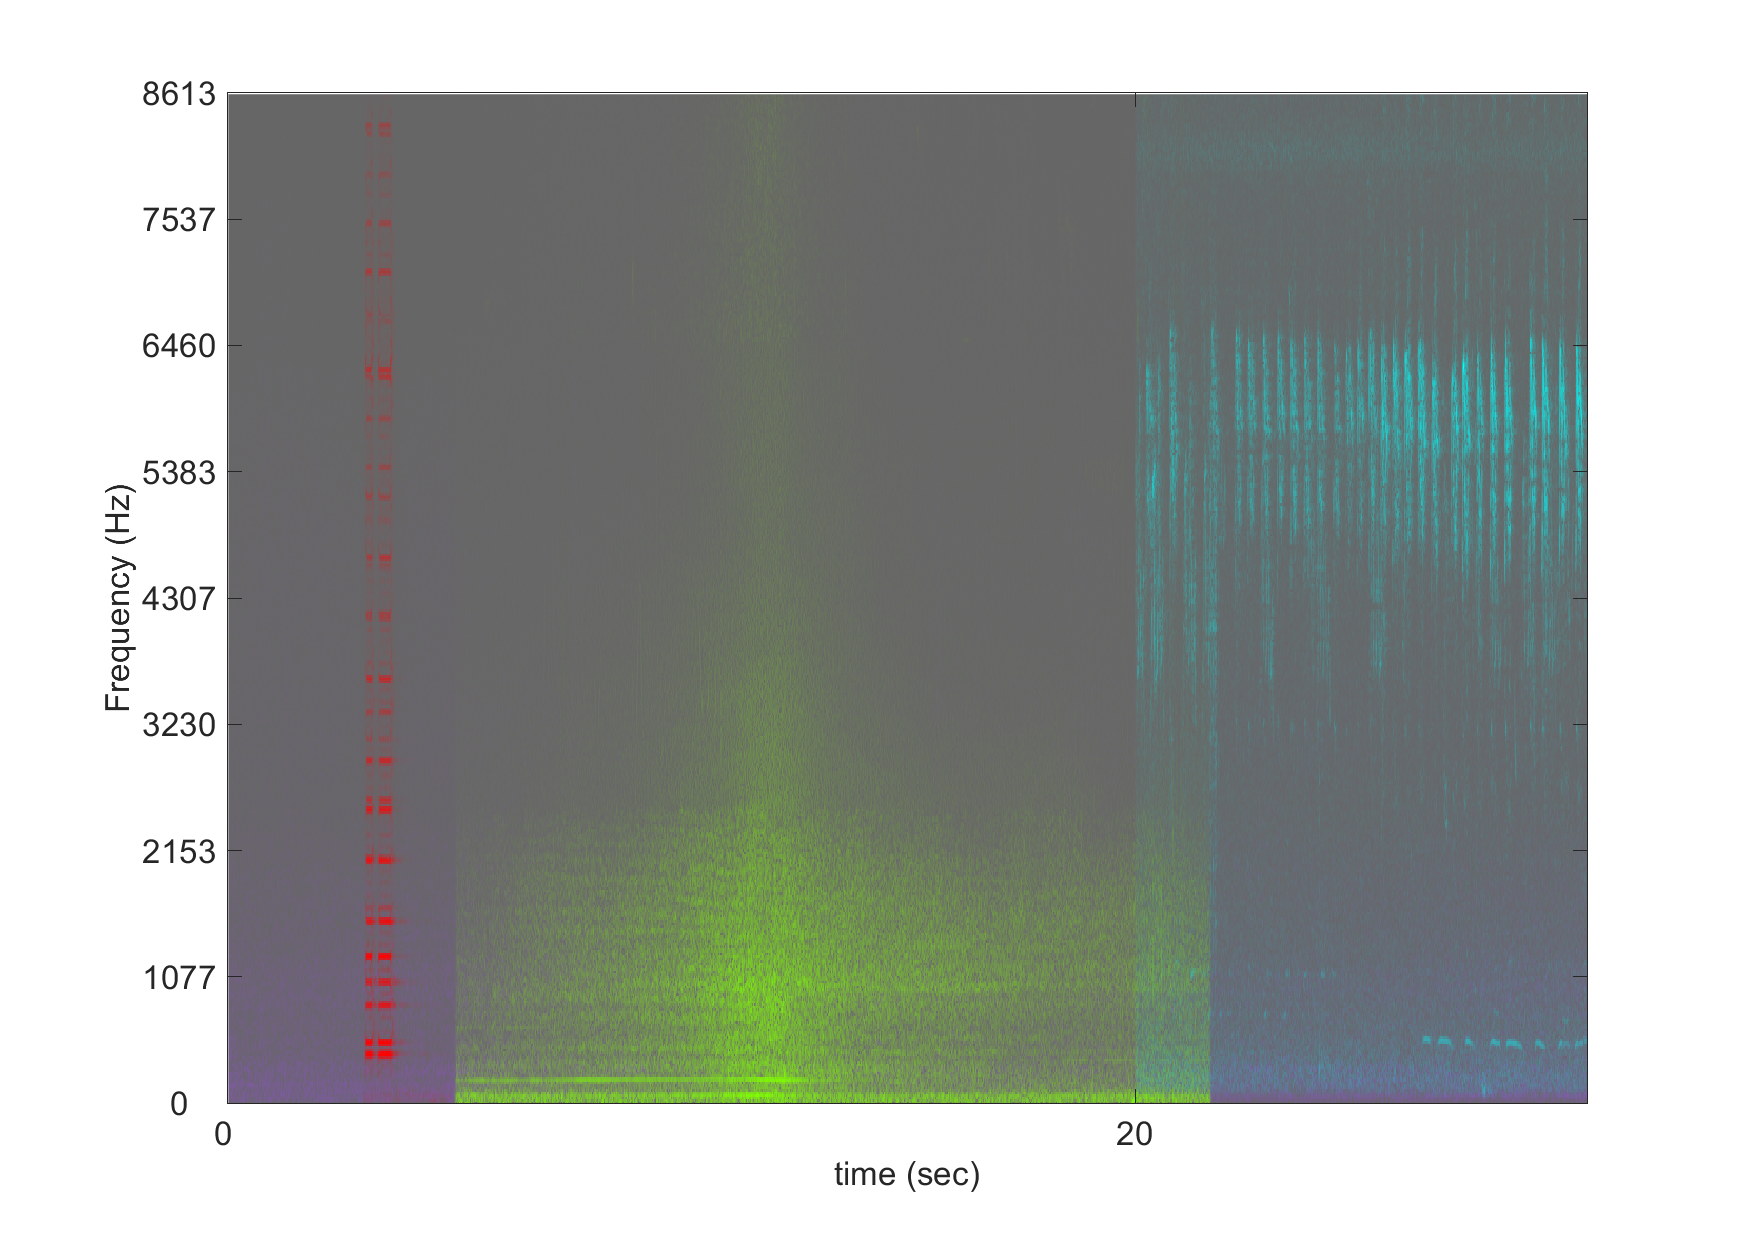
\includegraphics[width=\linewidth]{./figures/exempleSimScene3-spectrum.png}
       \caption{}
       \label{fig:simScene_spec}
    \end{subfigure}%
    \hfill
    \begin{subfigure}[t]{0.47\linewidth}
        \centering
       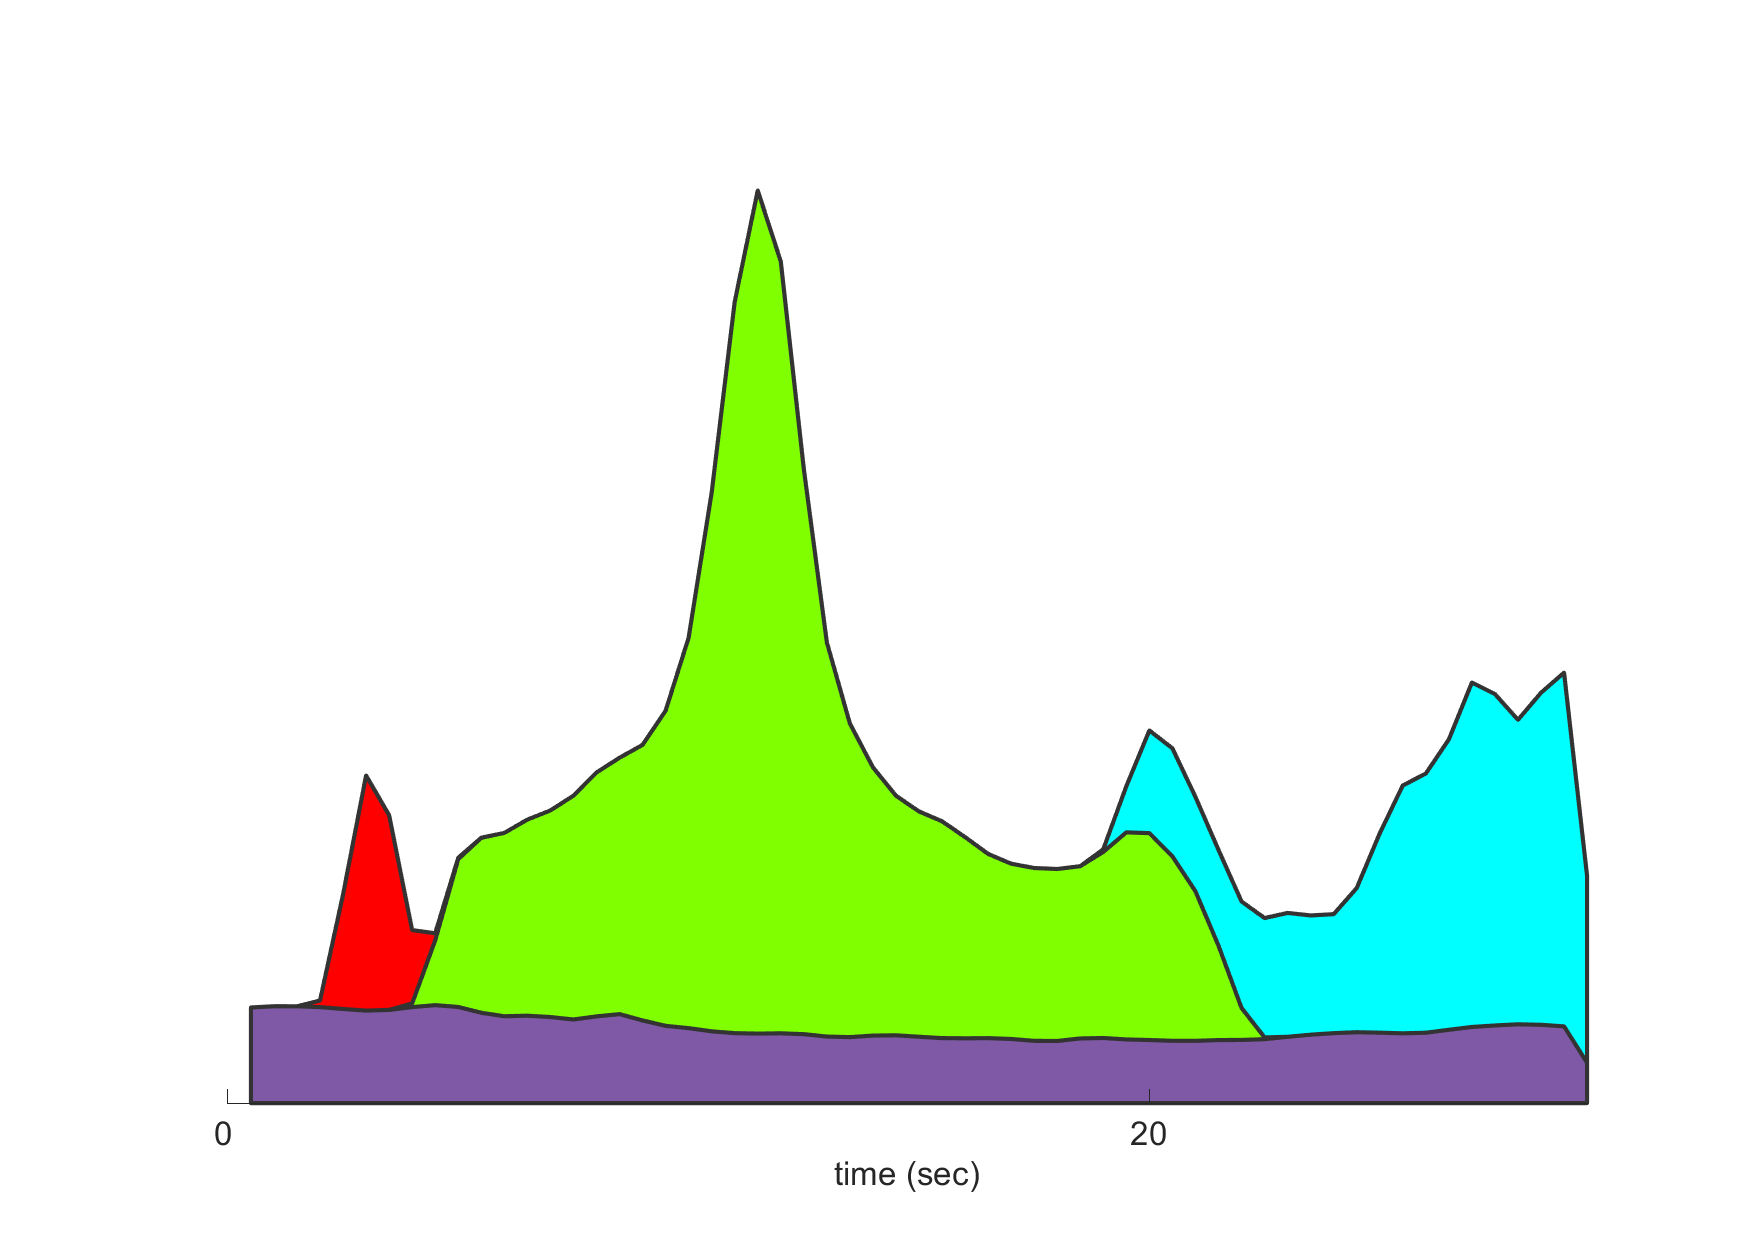
\includegraphics[width=\linewidth]{./figures/exempleSimScene3-timeDomain.png}
       \caption{}
       \label{fig:simScene_time}
    \end{subfigure}
    \caption{Example of a simple scene created with \textit{SimScene} software ((\ref{fig:simScene_spec}) the spectrogram, (\ref{fig:simScene_time}), the time domain}) with a sound background (road traffic in purple) and 3 sound events (car horn in red, car passage in green and whistling bird in blue):
    \label{fig:example_simScene}
\end{figure}

This database enables creating realistic urban sound scenes from the road traffic point of view \cite{gloaguen_creation_2017}. A sound mixing corpus is composed of 6 sub-corpus of 25 audio files each lasting 30 seconds. Each sub-corpus is characterized by a specific generic sound class that summed with traffic will make the estimation of the traffic level more difficult. The classes are: \textit{alert} (car horn, siren), \textit{animals} (barking dog , whistling birds), \textit{climate} (wind, rain), \textit{humans} (crowd noise and voice), \textit{mechanics} (different metallic and construction site noises) and \textit{transportation} (train, tramway and plane). In each file, traffic component is present as the sum of the background and event traffic sounds and is mixed with the other sound classes. The sound classes that are not related to the traffic component are summed up as the \textit{interfering} sound class. To test different scenarios, each audio file is duplicated with the traffic sound level of the entire sound scene, $L_{p,traffic}$, fixed to a specific level according to the sound level of the \textit{interfering} class, $L_{p,interfering}$,  following the relation (\ref{eq:tir}).

\begin{equation}\label{eq:tir}
TIR = L_{p,traffic}-L_{p,interfering}
\end{equation}

with the \textit{Traffic Interference Ratio} $TIR = \left[-12, -6, 0, 6, 12\right]$. When $TIR = -12$, the traffic component is then less present than the interfering class. When $TIR = 12$ it is the opposite: the trafffic class is louder than the interfering class. The total number of scenes designed is 750 (6 sub-corpus $\times$ 25 scenes $\times$  5 $TIR$ values).

\subsection{Experiment}

The experiment consists in estimating the traffic road sound level of the 6 environmental sound sub-corpus (\textit{alert} (al), \textit{animals} (an), \textit{humans} (hu), \textit{climate} (cl), \textit{mechanics} (me), \textit{transportation} (tr)) and for 5 $TIR$ ([-12 -6 0 6 12] dB). The spectrogram $\mathbf{V}$ of each sound is built with a window size $w = 2^{12}$ with a 50 $\%$ overlap and a number of point $nfft = 2^{12}$ ($N$ = 644).

The first estimator to determine the traffic sound level is a frequency low-pass filter which depends only on the cut-off frequencies $f_c$ = [500 1k 2k 5k 10k 20k] Hz (see Figure \ref{fig:bloc_filtre}). The spectrogram $\mathbf{V}$ is filtered and the remaining energy is then considered as traffic component (eq. \ref{eq:v_tr_filtered}),

\begin{equation}\label{eq:v_tr_filtered}
\mathbf{\tilde{V}}_{traffic} = \mathbf{V}_{f_c}.
\end{equation}

The second estimator is the proposed scheme, based on several flavors of the NMF framework. Multiples experimental factors are involved here between the dictionary learning and NMF (see Figure \ref{fig:bloc_nmf}).

\begin{figure}

    \centering
    \begin{subfigure}[t]{0.45\textwidth}
        \centering
        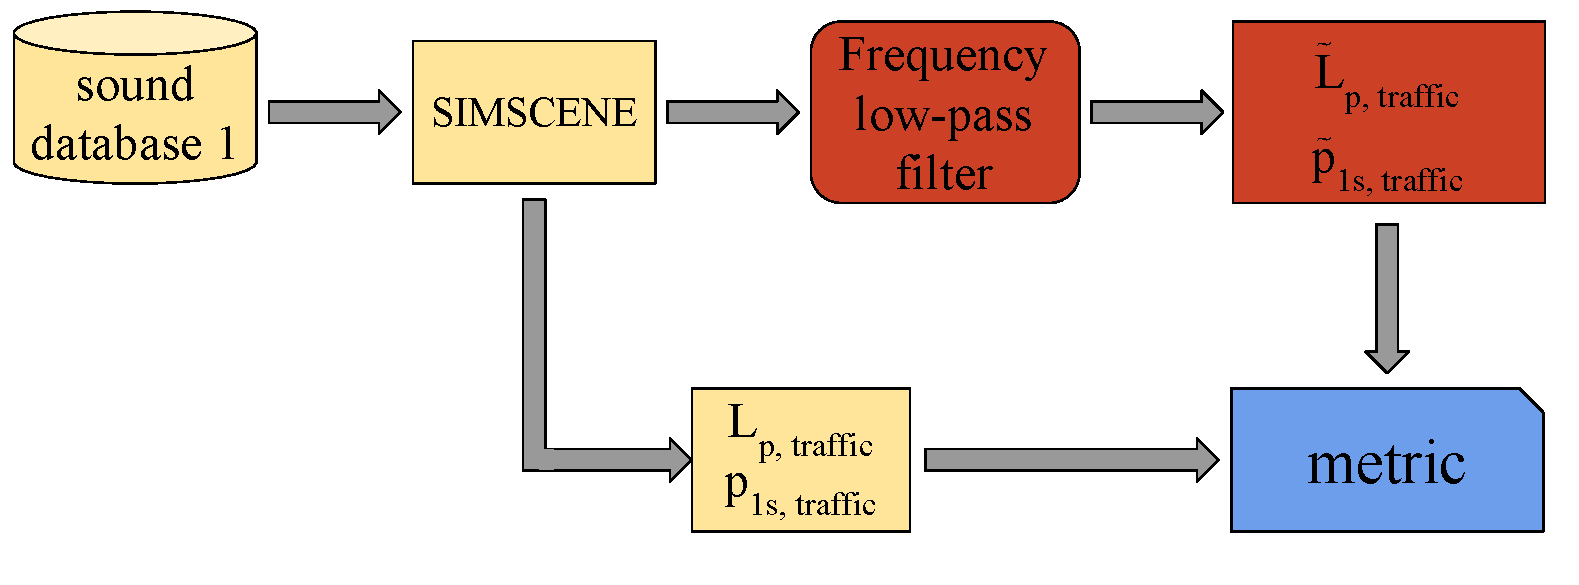
\includegraphics[width=\linewidth]{figures/bloc_diagram_filtrage_EN.pdf}
  		\caption{}
  		\label{fig:bloc_filtre}
    \end{subfigure}%
    \vfill
    \begin{subfigure}[t]{0.45\textwidth}
        \centering
        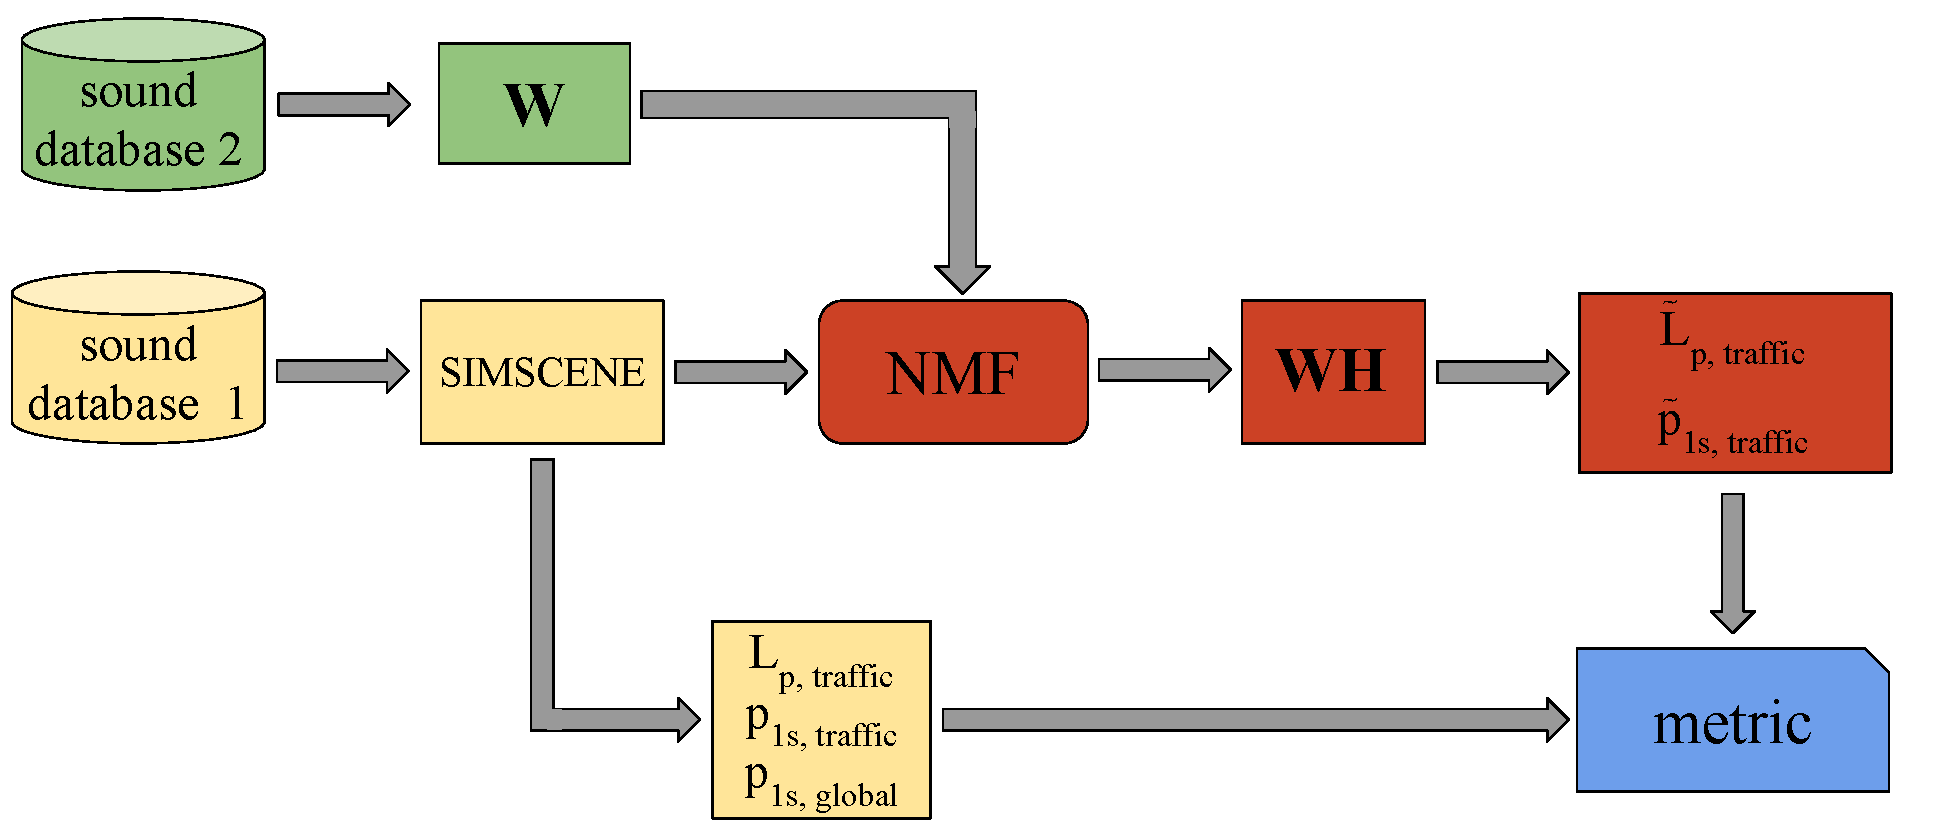
\includegraphics[width=\linewidth]{figures/bloc_diagram_NMF_EN.pdf}
		\caption{}
		\label{fig:bloc_nmf}
    \end{subfigure}

    \caption{Block diagrams summed up the different step of the process for the frequency low-pass filter (a) and for NMF (b)}
\end{figure}

\begin{table*}[t]
\centering
\begin{tabular}{lcccccc}
\textbf{Experimental factors} &  \multicolumn{6}{c}{value}\\ \toprule
$\mathbf{K}$ & 25 & 50 & 100 & 200 & & \\
\rowcolor[HTML]{EFEFEF}
$\mathbf{w_t}$ (s)& \multicolumn{2}{c}{0.5} & \multicolumn{2}{c}{1}  & \multicolumn{2}{c}{\textit{all}} \\
$\mathbf{TIR}$ (dB) & -12 & -6 & 0 & 6 & 12 &  \\
\rowcolor[HTML]{EFEFEF}
\textbf{sub-classes} & alert & animals & climate & humans & transportation & mechanics \\
$\mathbf{\beta}$ & \multicolumn{3}{c}{1} & \multicolumn{3}{c}{2} \\
\rowcolor[HTML]{EFEFEF}
$\mathbf{f_c}$ (kHz) & 0.5 & 1 & 2 & 5 & 10 & 20 \\
\textbf{method} & \multicolumn{2}{c}{filter} & SUP NMF & S-S NMF & TI NMF \\
\rowcolor[HTML]{EFEFEF}
$\mathbf{t}$ & \multicolumn{6}{c}{0.20:0.01:0.70} \\ \bottomrule
\end{tabular}
\caption{Summary of the different experimental factors taken into account in the frequency low-pass filter and NMF process and their values for the estimation of the traffic sound level}
\label{tab:experimental_factors}
\end{table*}


\subsubsection{Dictionary building}\label{part:dictionary_learning}

The dictionary is built from a second sound database dedicated specifically to this task. It is composed of 53 audio files of passing cars. These records have been made on the Ifsttar's runway too with the same experimental conditions that the records made for the \textit{SimScene} database but with two different cars (Dacia Sandero and Renault Clio). First, for each audio file, its spectrogram is calculated with fixed parameters ($w$, 50 $\%$ overlap, $nfft$). Then time/frequency windows of $F \times w_t $ dimension are applied without overlapping on the spectrogram in order to consider several spectrum for each audio file. $w_t$ is fixed at $wt = [0.5~1]$ second. In each window, the root mean square value is calculated on each frequency bin to reduce the windowed spectrogram in one spectra of $F \times 1$ dimension.  A special case is added where the root mean square of \textit{all} the spectrogram is applied (each audio file generates one element $k$ of $\mathbf{W}$). An example that illustrates the process can be found on Figure \ref{fig:spec_elementW} on a 3 second extract of the spectrogram of a car passage ; see Figure \ref{fig:specW}. In the case where $w_t$ = 1 second , 3 elements are therefore extracted from the spectrogram while in the case where $w_t$ = \textit{all}, all the spectrogram is reduced to one element ; see Figure \ref{fig:ElementW}.

\begin{figure}[t!]
    \centering
    \begin{subfigure}[t]{0.47\linewidth}
        \centering
       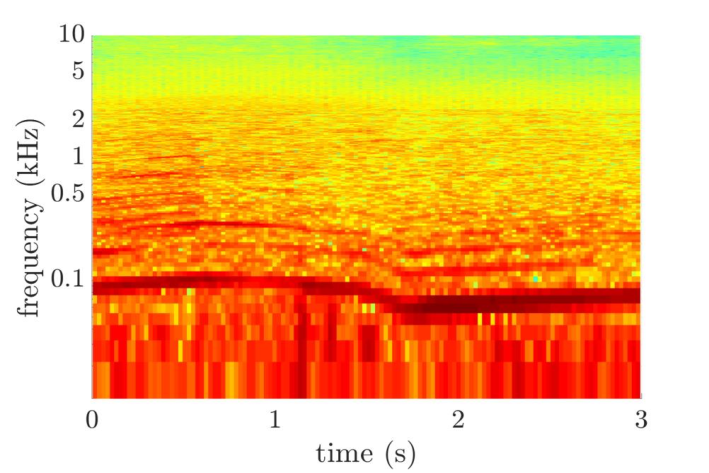
\includegraphics[width=\linewidth]{figures/dictionary1.pdf}
       \caption{}
        \label{fig:specW}
    \end{subfigure}%
    \hfill
    \begin{subfigure}[t]{0.47\linewidth}
        \centering
       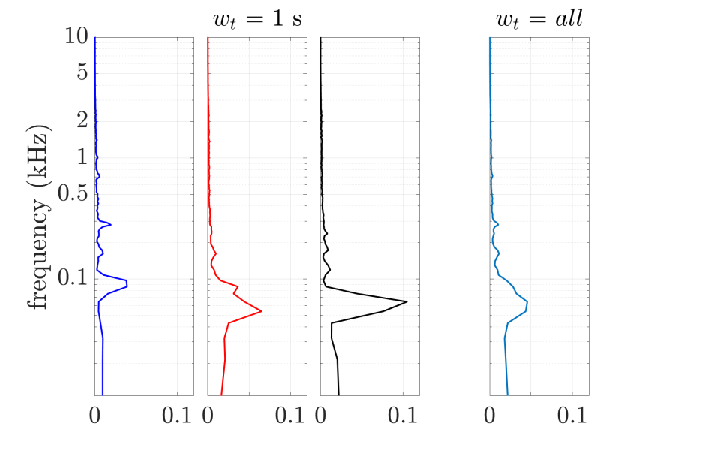
\includegraphics[width=\linewidth]{figures/dictionary2.pdf}
        \caption{}
        \label{fig:ElementW}
    \end{subfigure}
    \caption{Example of the dictionary building with a 3 second extract of a car passage (\ref{fig:specW}). With $w_t$ = 1 second, 3 spectrum are generated and included in $\mathbf{W}$ while for $w_t$ = $all$, the audio file is resume to 1 spectra (\ref{fig:ElementW}).}
    \label{fig:spec_elementW}
\end{figure}

Since the number of elements given by this processing can be high, in order to reduce the computational time and delete redundant information, a $K$-means clustering is applied to reduce the number of spectrum to $K = \left[ 25, 50, 100, 200\right]$.

The obtained dictionary is expressed with third octave bands and each basis vector of $\mathbf{W}$ is normalized such as $\vert \vert \mathbf{W_k} \vert \vert = 1$ with $\vert \vert \bullet \vert\vert$ the $\ell$-1 norm. Table \ref{tab:experimental_factors} summarizes the experimental factors ($K$ and $w_t$) for the dictionary building and their related values.

\subsubsection{Experimental factors of NMF}

SUP and S-S NMF are performed for 400 iterations which is sufficiently enough to get a stabilized reconstruction. TI NMF is performed on a lower number of iteration (60) to prevent $\mathbf{W}$ to not deviate too much from the initial dictionary.

The spectrogram $\mathbf{V}$ and the dictionary $\mathbf{W}$ are expressed with third octave bands ($F$ = 29). This coarser method allows the matrix reduction and decrease the computation time. But,  must of all, by expressing the frequency axis on a log frequency axis,  the low frequencies, where the traffic energy is focused, are described more finely than the high frequencies. The case of a linear frequency axis has been investigated and offer similar results which were not better.

For TI NMF, the threshold is define between 0.20 and 0.70 with a 0.01 step. Table \ref{tab:experimental_factors} summarizes the experimental factors and their related values.

\begin{table*}[t]
\centering
\begin{tabular}{@{}cccccc@{}}
\toprule
\textbf{method} & $\mathbf{\beta}$ & $\mathbf{K}$ & $\mathbf{w_t}$ (s) &   $\mathbf{t}$ & \textbf{$MAE$ (dB)} \\ \midrule
filter 20 kHz &  &  &  &  & 4.69 ($\pm$ 4.52) \\
filter 0.5 kHz&  &   &  &  & 2.89 ($\pm$ 2.84) \\ \hline \hline
SUP NMF &  1 & 50 & 0.5  &  & 3.44 ($\pm$ 3.70) \\
SUP NMF &  2 & 50 & 0.5  &   & 3.02 ($\pm$ 3.33) \\ \hline \hline
S-S NMF &  1 & 100 & 0.5 &   & 2.33 ($\pm$ 1.10) \\
S-S NMF &  2 & 100 & 0.5 &   & 2.32 ($\pm$ 1.26) \\ \hline \hline
TI NMF &  1 & 200 & 0.5 &  0.42 &\textbf{2.19 ($\pm$ 2.18)} \\
TI NMF &  2 & 25 & all &  0.54 & 2.20 ($\pm$ 2.26)\\ \bottomrule
\end{tabular}
\caption{Best results according to $\beta$ and \textit{method} experimental factors, in bold letter, the lowest error.}
\label{tab:results}
\end{table*}

\begin{table*}[t]
\centering
\begin{tabular}{@{}cccccc@{}}
\toprule
\textbf{method} & filter & filter & SUP NMF & S-S NMF & TI NMF \\ \midrule
$f_c$ (kHz) & 20 & 0.5 & 20 & 20 & 20 \\
$\mathbf{\beta}$ &  &  & 2 & 2 & 1 \\ \hline
\textbf{-12} & 12.25 ($\pm$ 0.05) & 7.36 ($\pm$ 3.00) & 8.65 ($\pm$ 1.88) & 3.88 ($\pm$ 1.52) & 5.35 ($\pm$ 2.71) \\
\textbf{-6} & 6.96 ($\pm$ 0.05) & 3.44 ($\pm$ 1.65) & 4.22 ($\pm$ 1.27) & 1.37 ($\pm$ 0.71)  & 2.82 ($\pm$ 1.30) \\
\textbf{0} & 3.00 ($\pm$ 0.03) & 1.17 ($\pm$ 0.24) & 1.34 ($\pm$ 0.56) & 1.11 ($\pm$ 0.25) & 1.26 ($\pm$ 0.35) \\
\textbf{6} & 0.25 ($\pm$ 0.06) & 1.03 ($\pm$ 0.26) & 0.26 ($\pm$ 0.10) & 2.25 ($\pm$ 0.19) & 0.70 ($\pm$ 0.32) \\
\textbf{12} & 0.26 ($\pm$ 0.00) & 1.45 ($\pm$ 0.13) & 0.64 ($\pm$ 0.06) & 2.96 ($\pm$ 0.21)  & 0.84 ($\pm$ 0.24) \\ \bottomrule
\end{tabular}
\caption{$MAE$ error averaged on all sub-classes on each $TIR$ for the best scenario according to each method}
\label{tab:results_TIR}
\end{table*}


\subsubsection{Metrics}
The performances of the two estimators (filter and NMF) of the road traffic sound level are assessed through the calculation of one metric, the Mean Absolute Error ($MAE$). It expresses the quality of the long-term reconstruction of the signal and consists in the average over the $M$ sound scenes of the absolute difference between the exact and estimated traffic sound level in dB,

\begin{equation}
MAE = \frac{\sum_{m = 1}^M\vert L^m_{p,traffic}-\tilde{L}^m_{p,traffic} \vert}{M}.
\end{equation}

In all, according Table \ref{tab:experimental_factors}, 24540 settings are performed between the different form of the dictionary $\mathbf{W}$ and the multiple experimental factors taken into account by NMF. For the filter estimator, between the $TIR$, the sub-classes and $f_c$, 180 settings are performed whereas for SUP and S-S NMF, 3780 associations of factors are made. For TI NMF, 8400 combinations can be calculated.

\section{Results}\label{part:results}

Table \ref{tab:results} summarized, according to the 2 main factors (\textit{method}, $\beta$), the $MAE$ error averaged on all sub-classes and all $TIR$ (750 sound mixtures in all). For the low-passa frequency filters and each NMF approaches, the best parameter combinations are detailed according to the $TIR$ in Table \ref{tab:results_TIR},  and are expand to the sub-classes in Figures \ref{fig:TIR_class_filter}, \ref{fig:TIR_class_sup}, \ref{fig:TIR_class_semi} and \ref{fig:TIR_class_TI}. \\

First, the errors produced by the filter are detailed. $f_c = 20 $ kHz is equivalent to consider all the sound mixtures without distinction between traffic and others sound sources. Consequently, in low $TIR$ (-12 dB and -6 dB), where traffic component is scarce, the error is more important than in high $TIR$ (6 dB and 12 dB) where the traffic component is predominant. $f_c = 500$ Hz is the cut-off frequency with the lower mean error obtained. It is then the first baseline to use to compare the performances of NMF.

In low $TIR$, for \textit{alert} and \textit{animals}, sub-classes composed of higher frequencies, this filter is efficient as it removes these frequency components. For the other sub-classes where low frequency contents are present (storm for \textit{climate}, voices in \textit{humans}, planes, tramway and train in \textit{transport} and ventilation noise in \textit{mechanics}), the filter considers all the energy located in the pass-band and then do not dissociate the traffic element from the other sound sources. The errors are then nearly all superior to 4 dB and are overestimate ; see Figure \ref{fig:alert_-12}. In opposite, in high $TIR$, the error is due to the energy removed from the traffic which has the consequence to underestimate the sound levels ; see Figure \ref{fig:alert_12}. The 500 Hz filter finds a balance between what it is put aside in low $TIR$ and what it is remained in high $TIR$. \\

\begin{figure*}[t]
    \centering
    \begin{subfigure}[t]{0.45\textwidth}
        \centering
        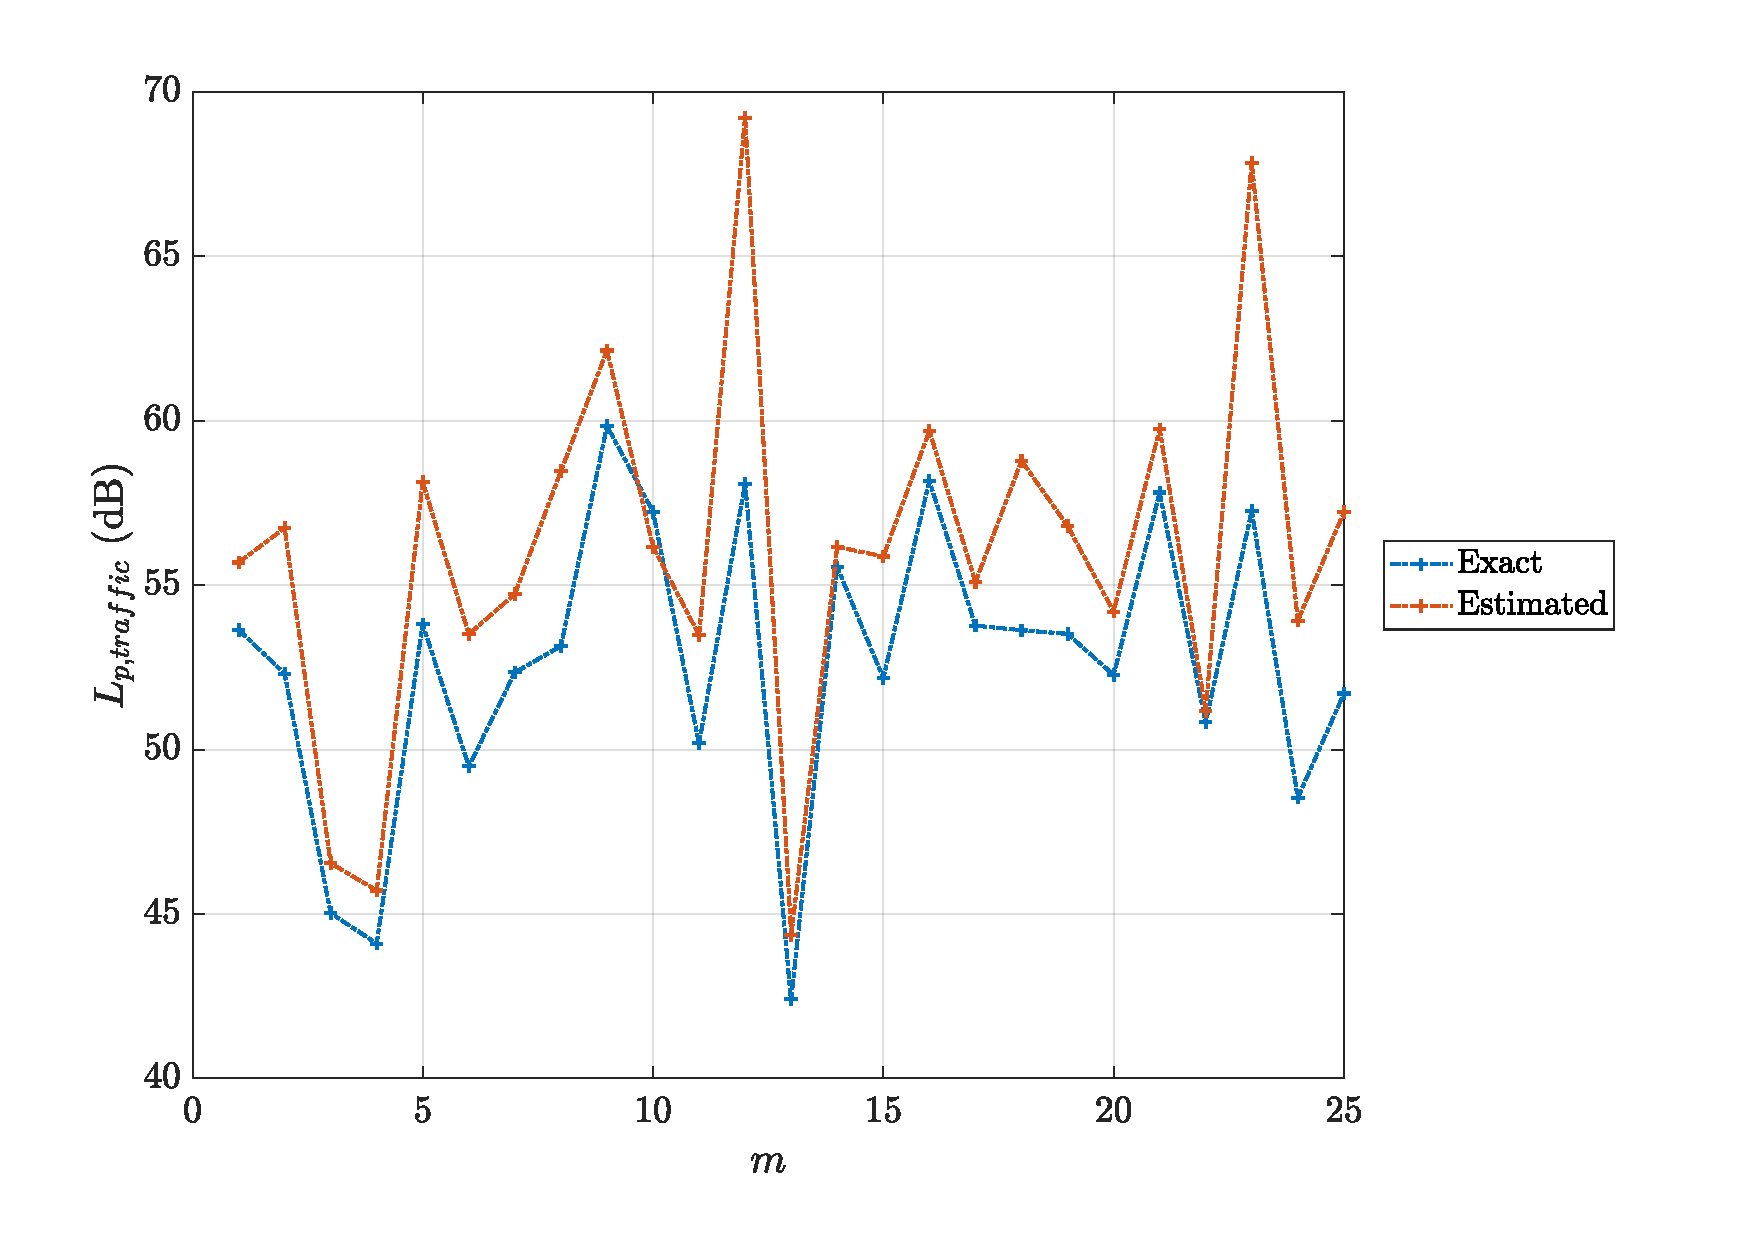
\includegraphics[width=\linewidth]{figures/LeqTrafficComparison_filter_alert_-12.pdf}
        \caption{}
        \label{fig:alert_-12}
    \end{subfigure}%
    \hfill
    \begin{subfigure}[t]{0.45\textwidth}
        \centering
        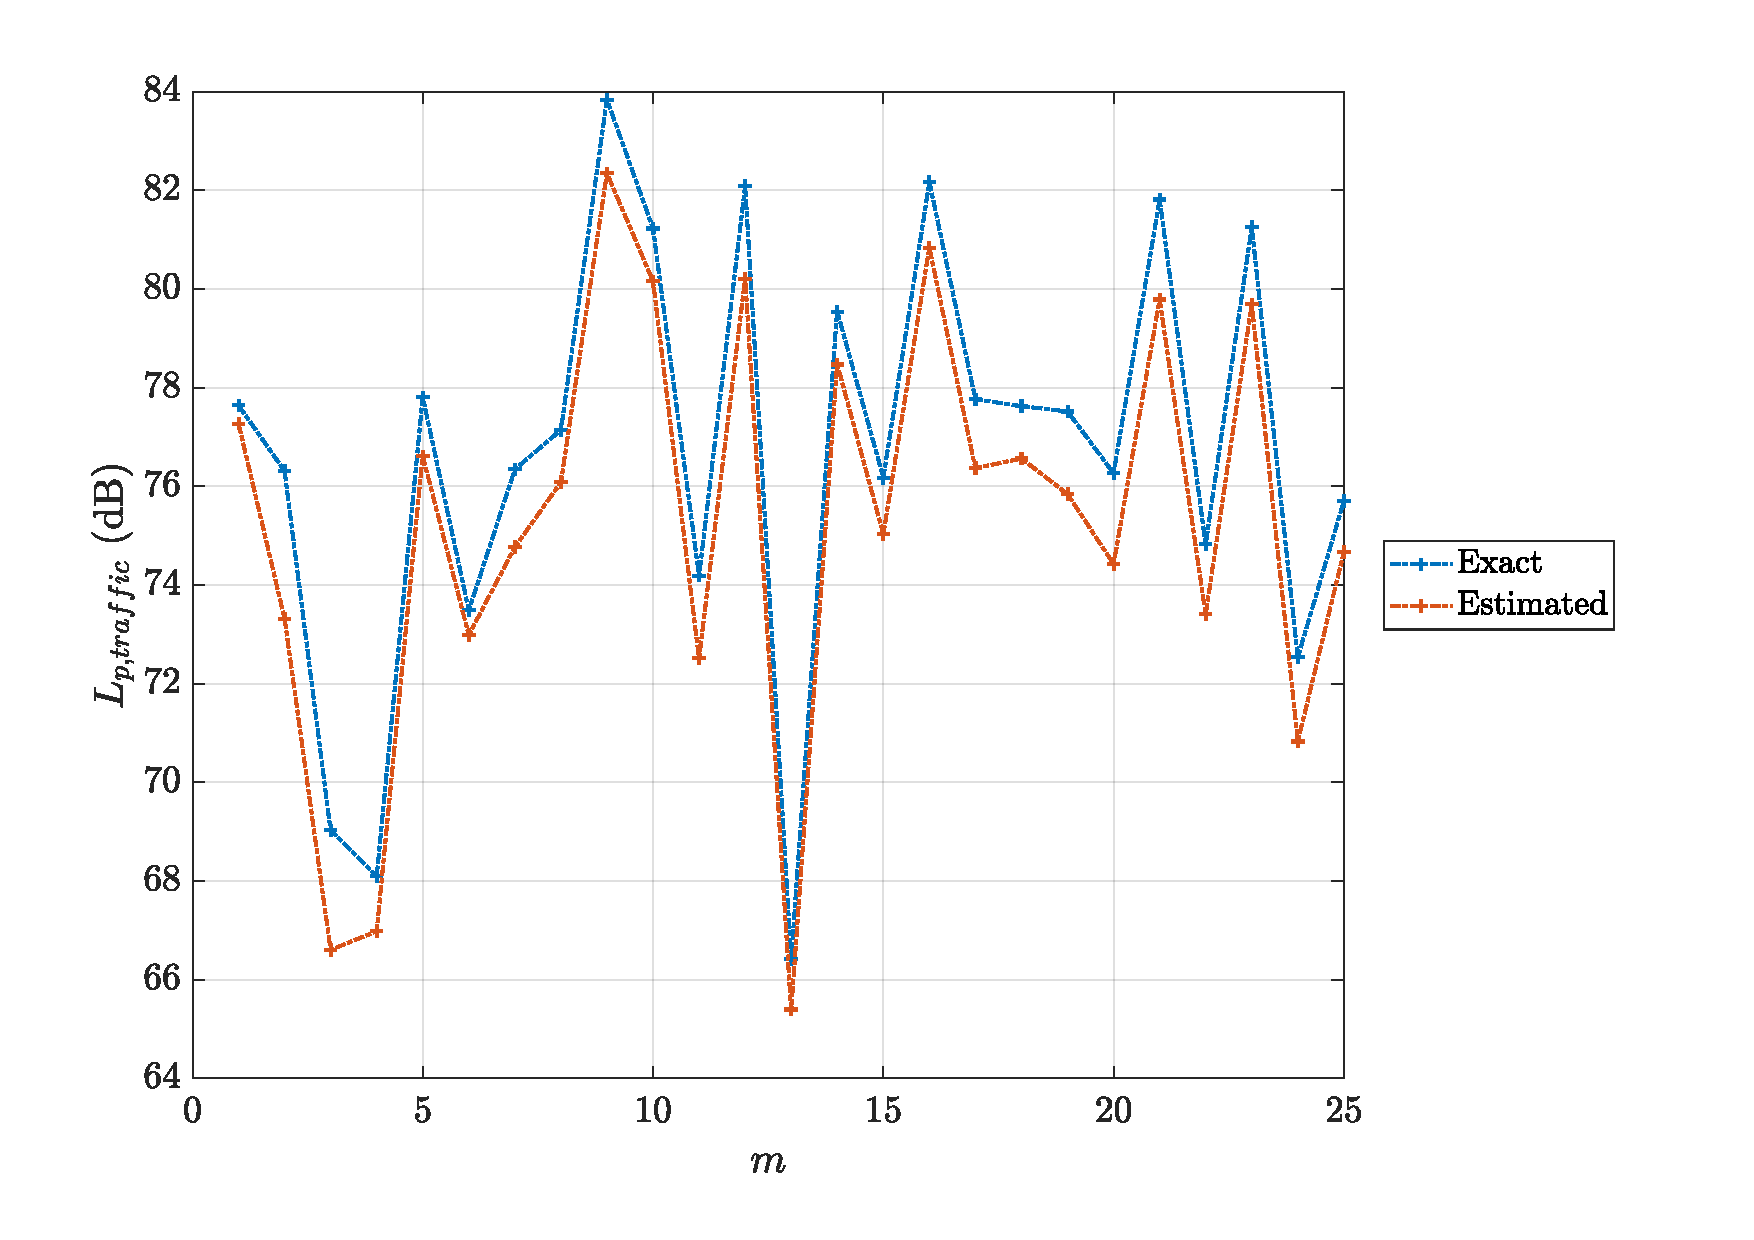
\includegraphics[width=\linewidth]{figures/LeqTrafficComparison_filter_alert_12.pdf}
        \caption{}
        \label{fig:alert_12}
    \end{subfigure}

    \caption{Global sound levels of the traffic estimated by the frequency low-pass filter with $f_c$ = 500 Hz for the sub-classes \textit{alert}: at $TIR = -12$ (\ref{fig:alert_-12}) and at $TIR$ (\ref{fig:alert_12}).}
    \label{fig:dictionaryExtraction}
\end{figure*}


Compare to the filter errors, the choice of some NMF approaches make it possible to decrease the road traffic sound level estimation. The supervised approach is the only method that has an average error superior to the 500 Hz filter baseline. Finally, it is the most sophisticated methods (S-S and TI NMF) that have better results. The lowest average error is obtained for TI NMF for $\beta$ = 1 and threshold $t$ = 0.42 with the dictionary factors $K$ = 200 and $w_t$ = 500 ms. On the other hand, the semi-supervised approach has a higher error but yet with a lower standard deviation.

\begin{figure*}[t]
    \centering
    \begin{subfigure}[t]{0.45\textwidth}
        \centering
        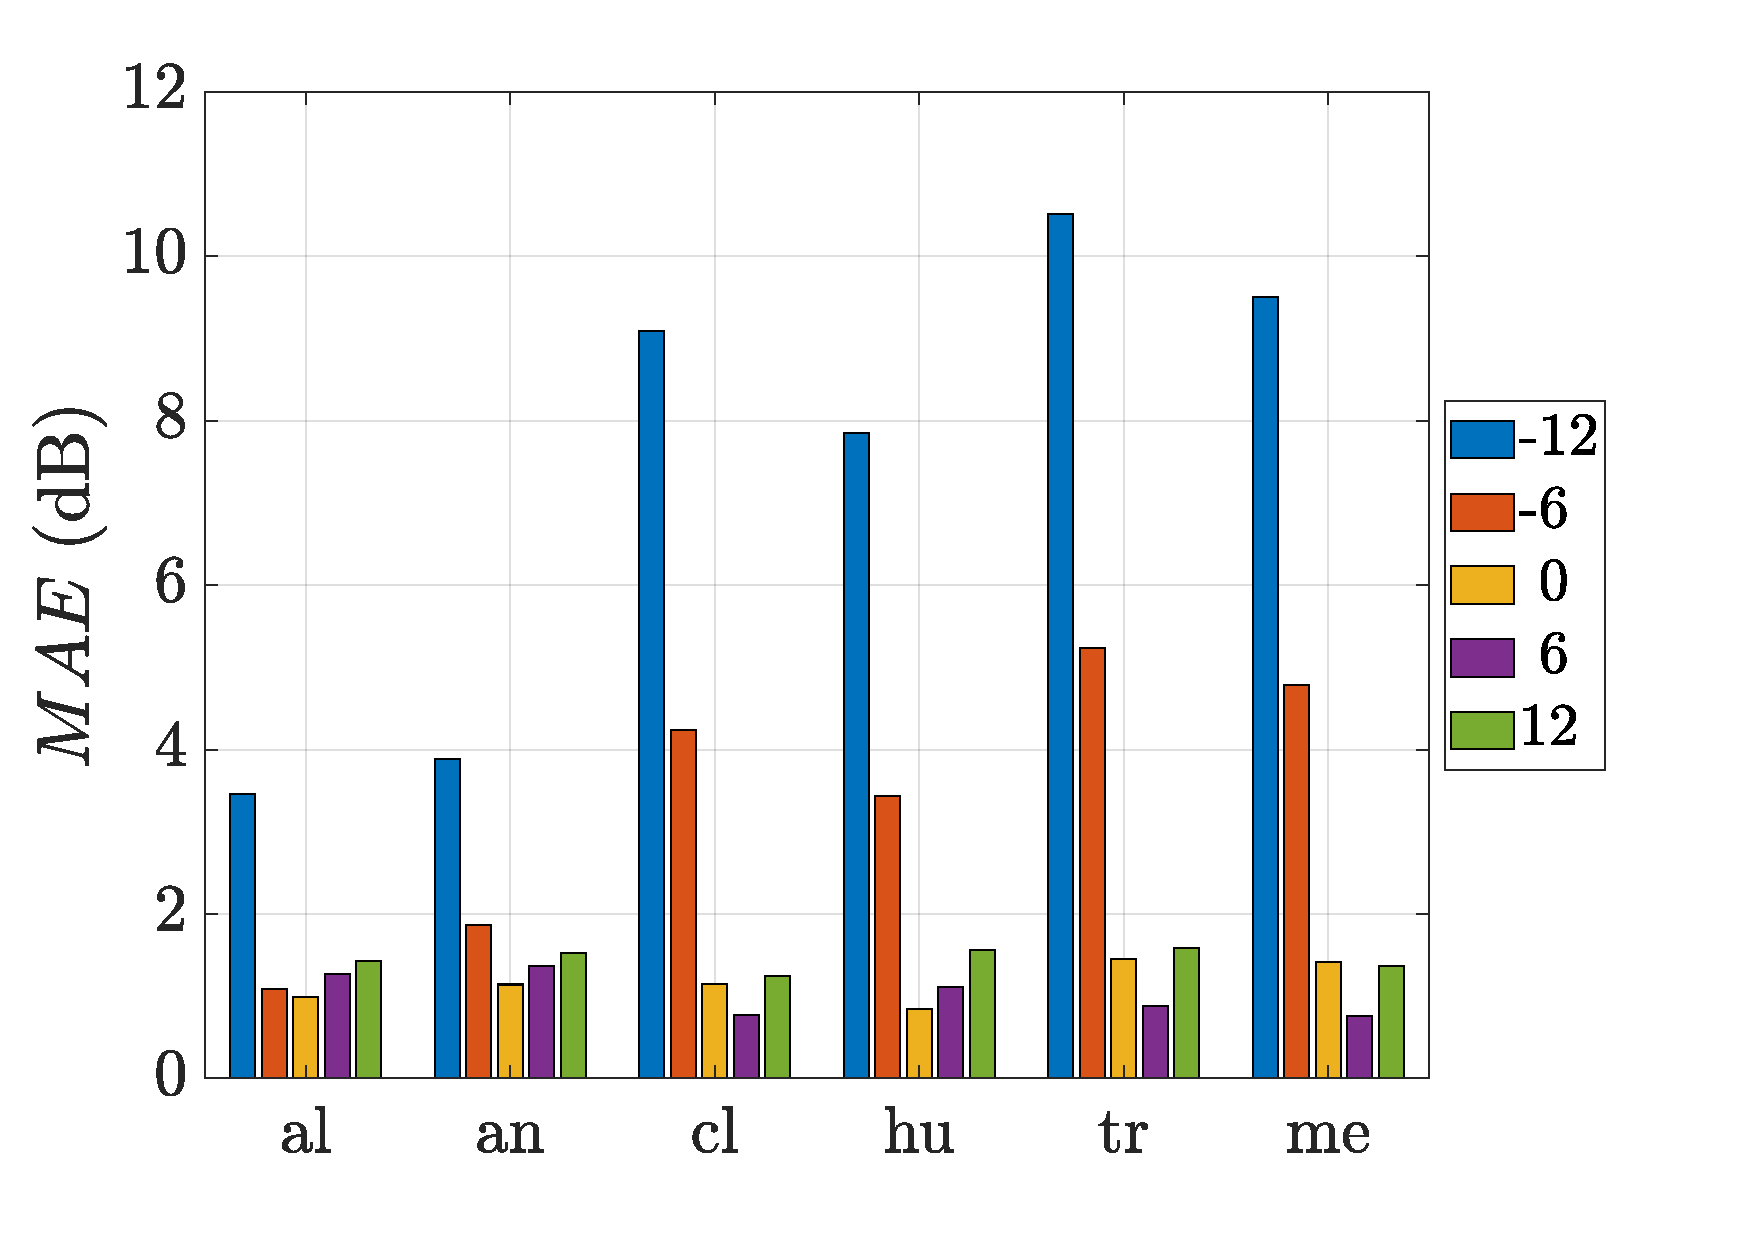
\includegraphics[width=\linewidth]{figures/filter_bar.pdf}
        \caption{Frequency low-pass filter with $f_c$ = 500 Hz}
        \label{fig:TIR_class_filter}
    \end{subfigure}%
    \hfill
    \begin{subfigure}[t]{0.45\textwidth}
        \centering
        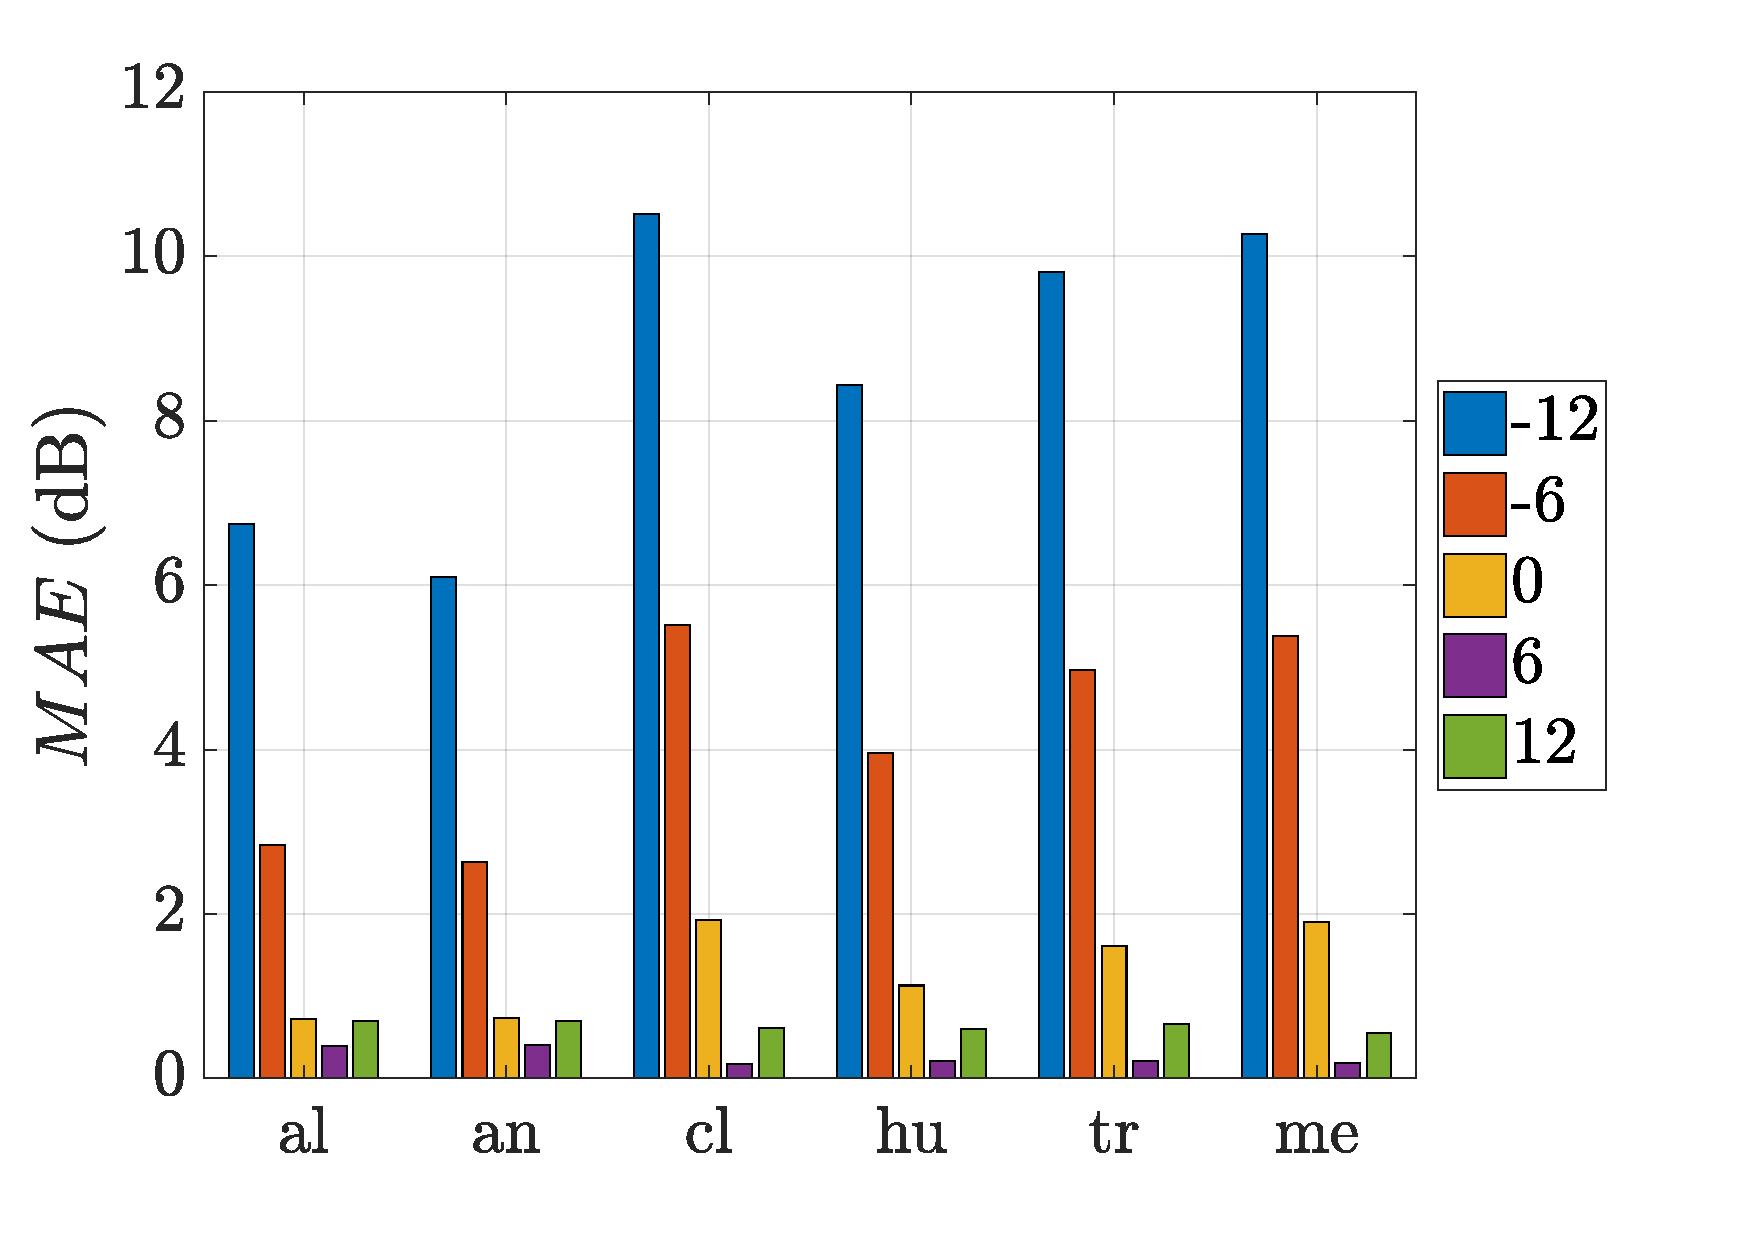
\includegraphics[width=\linewidth]{figures/sup_bar.pdf}
        \caption{$MAE$ error for each $TIR$ and sub-class with SUP NMF and $\beta$ = 2}
                \label{fig:TIR_class_sup}
    \end{subfigure}

    \begin{subfigure}[t]{0.45\textwidth}
        \centering
      	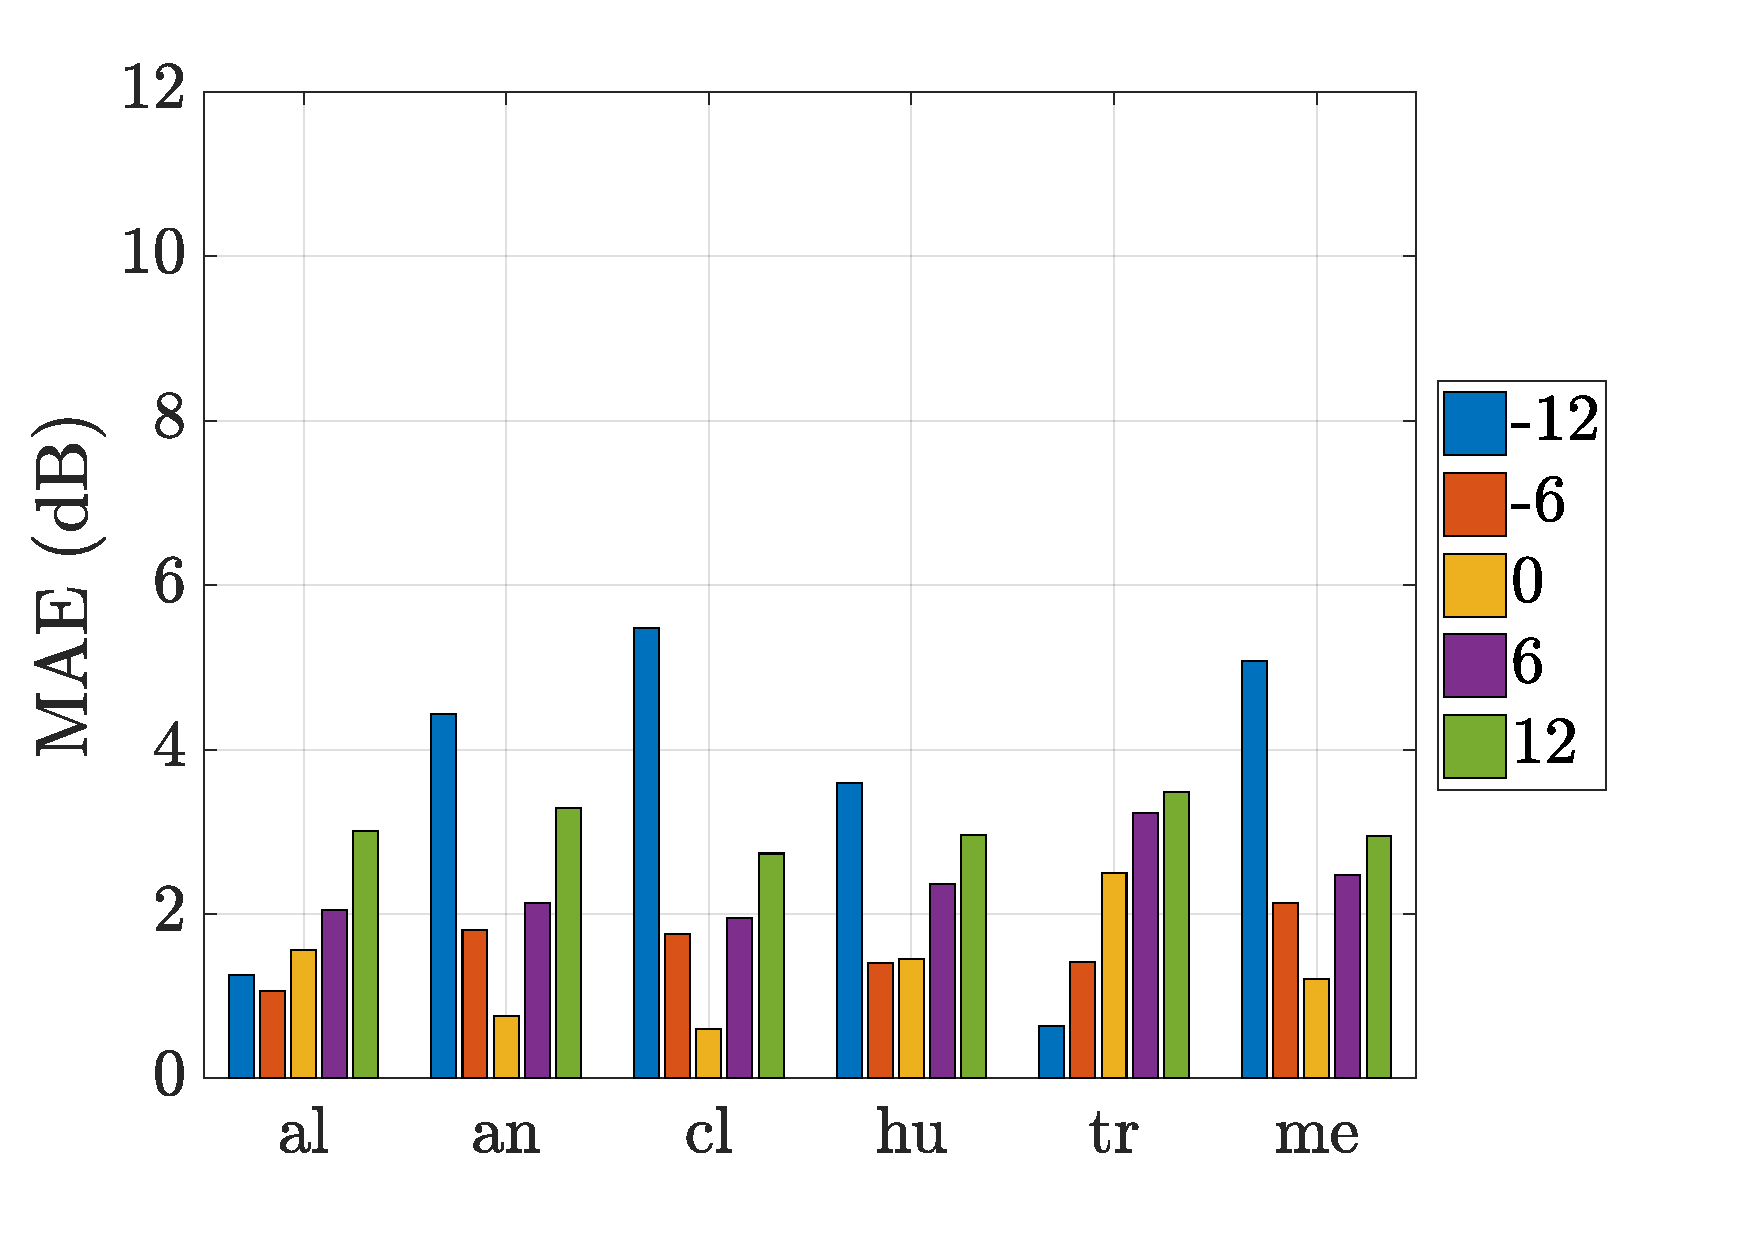
\includegraphics[width=\linewidth]{figures/semi-sup_bar.pdf}
        \caption{$MAE$ error for each $TIR$ and sub-class with S-S NMF and $\beta$ = 2}
                \label{fig:TIR_class_semi}
    \end{subfigure}%
    \hfill
    \begin{subfigure}[t]{0.45\textwidth}
        \centering
        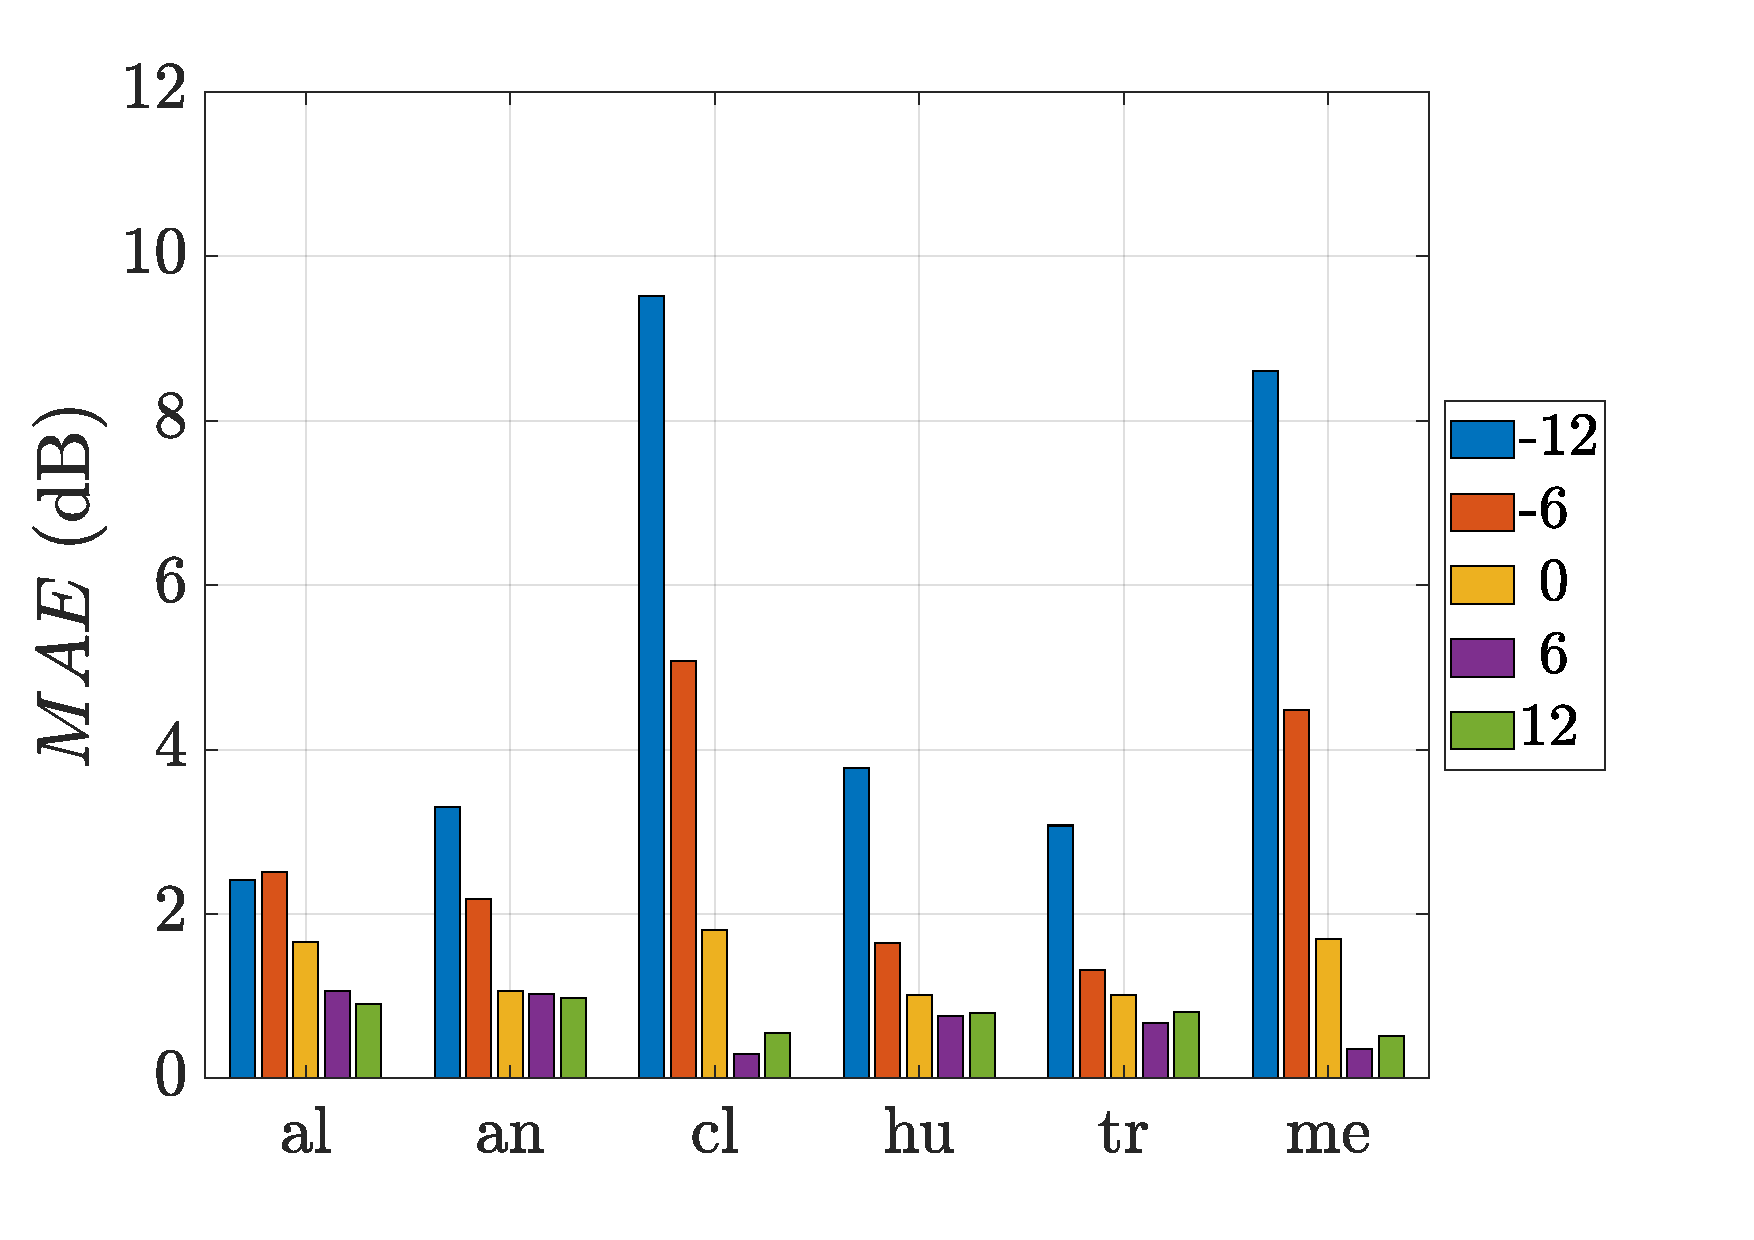
\includegraphics[width=\linewidth]{figures/TI_bar}
        \caption{$MAE$ error for each $TIR$ and sub-class with TI NMF, $\beta$ = 1 and $t$ = 0.42}
        \label{fig:TIR_class_TI}
    \end{subfigure}
    \caption{$MAE$ error for each sub-class and $TIR$ according to the the best results with the filter (\ref{fig:TIR_class_filter}) and each method (SUP (\ref{fig:TIR_class_sup}), S-S (\ref{fig:TIR_class_semi}) and TI (\ref{fig:TIR_class_TI} NMF))}
    \label{fig:TIR_bar}
\end{figure*}

According to Table \ref{tab:results_TIR} and Figures \ref{fig:TIR_bar}, the behavior between the 3 versions of NMF differs. In the case of SUP NMF, it fails to improve the filtering performances despite good results in high $TIR$.  the error are too important for low $TIR$ and this for all the sub-classes. This method reveals to be to rigid as $\mathbf{W}$ is composed of fixed traffic spectrum. In the case of low $TIR$, in the aim to reduce the objective function, see eq. \ref{eq:min-D-WH}, traffic elements are used whatever the sound event in the  sound scene. The case of a scene of the \textit{alert} sub-class is presented in Figure \ref{fig:lp_alert_-12}. Here when the car horn sounds, some elements of $\mathbf{W}$ are activated and are then considered as traffic component generating a wrong estimation of the sound level. This behavior disappear when the traffic component become predominant to the \textit{interfering} class, see Figure \ref{fig:lp_alert_12}. Thus composed the dictionary of only fixed traffic spectrum is not a sufficient way to estimate correctly the traffic sound level, $\tilde{L}_{p,traffic}$.

Consequently, with the add of a mobile part in the dictionary, $\mathbf{W_r}$, the semi-supervised approach  allows a better consideration of the \textit{interfering} class in low $TIR$. It brings a significant decrease of the errors for low $TIR$ as it can be see in Figure \ref{fig:TIR_class_semi}. The $\mathbf{W_r}$ composition, in the case of an \textit{alert} sub-class, is displayed in Figure \ref{fig:Y_alert-12} and this shows that the interfering class is easily integrated. The first element is mainly composed of high frequency bands which correspond to the car horns of the scene. This composition impacted directly the traffic sound level estimation as it can be seen in Figure \ref{fig:lp_alert_-12} where the traffic basics are no longer activated when the car horn sounds.

\begin{figure*}[t]
    \centering
    \begin{subfigure}[t]{0.45\textwidth}
        \centering
        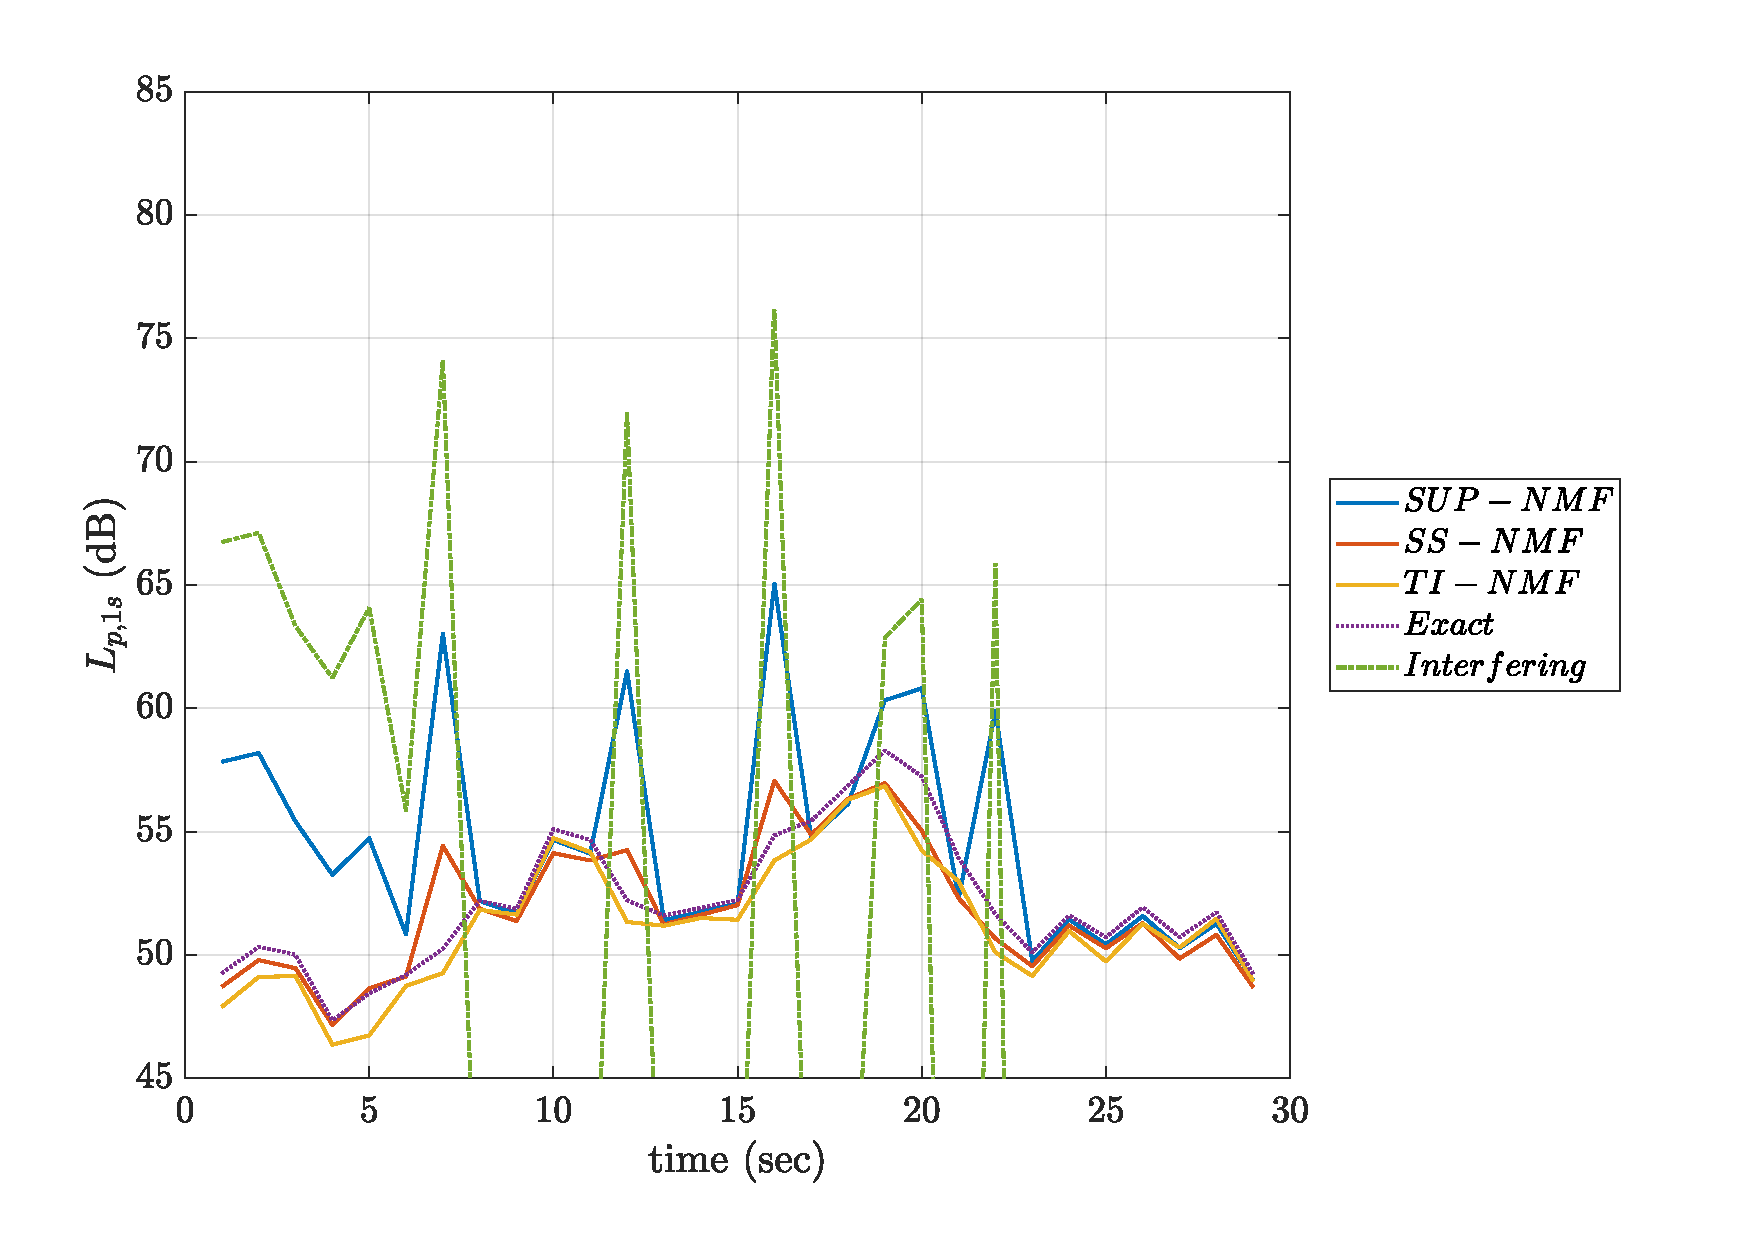
\includegraphics[width=\linewidth]{figures/NMF_Lp_alert-12.pdf}
        \caption{}
        \label{fig:lp_alert_-12}
    \end{subfigure}%
    \hfill
    \begin{subfigure}[t]{0.45\textwidth}
        \centering
        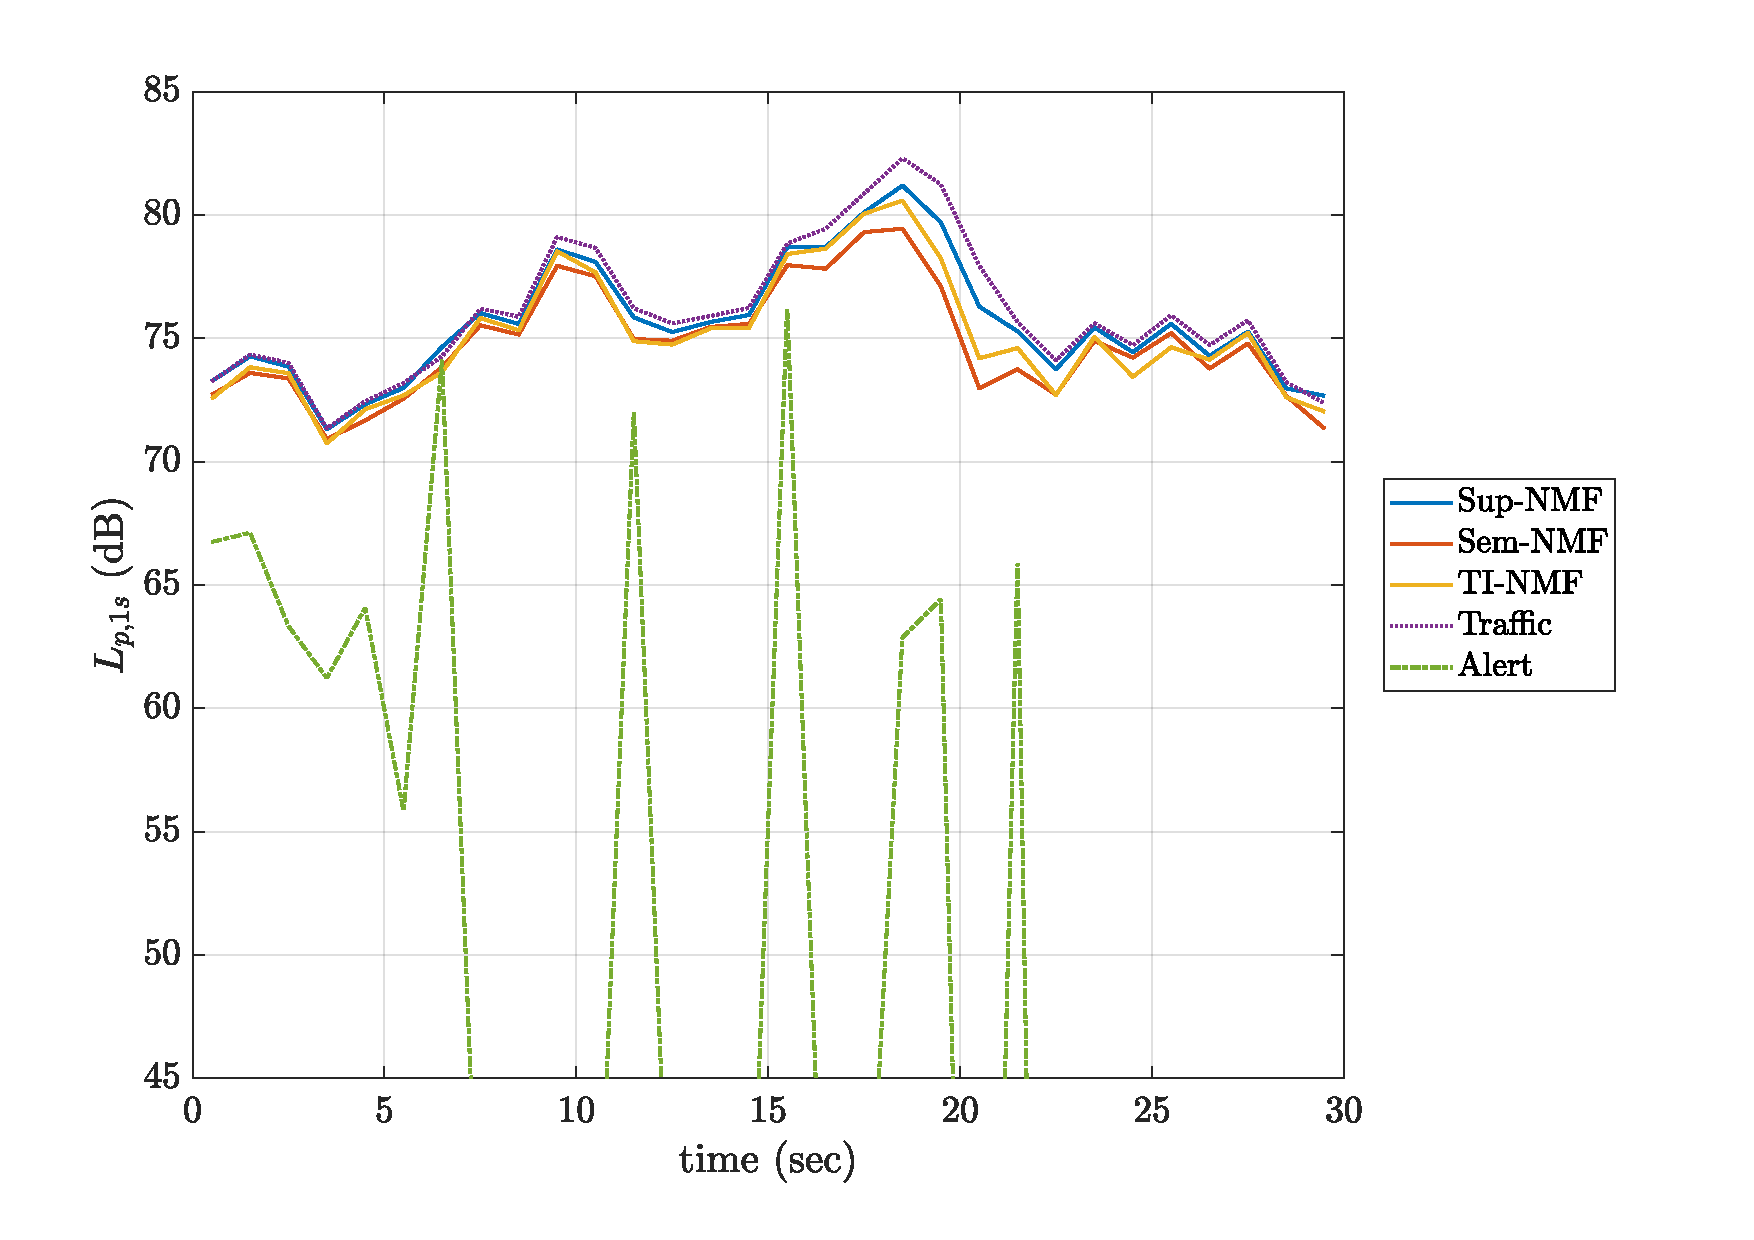
\includegraphics[width=\linewidth]{figures/NMF_Lp_alert12.pdf}
        \caption{}
        \label{fig:lp_alert_12}
    \end{subfigure}

    \caption{1 second equivalent sound pressure level of an \textit{alert} sub-class scene for : at $TIR = -12$ (\ref{fig:lp_alert_-12}) and at $TIR$ (\ref{fig:lp_alert_12}).}
    \label{fig:lp_alert}
\end{figure*}

However, the degrees of freedom of S-S NMF are restrictive for high $TIR$ as the errors exceed 2 dB for all sub-classes and increase with $TIR$ = 6 dB and 12 dB. Indeed, in order to reduce $D(\mathbf{V} \vert \vert \mathbf{WH}$), without constraint, S-S NMF is free to include traffic components in $\mathbf{W_r}$. Consequently, this behavior decreases the quality of the reconstruction of the traffic component. In Figure \ref{fig:Y_alert_12} for $TIR=12$ dB, the high frequency components of car horn have disappeared for the benefit of low frequency content. Consequently, the traffic sound level estimation is then underestimate as in Figure \ref{fig:lp_alert_12}. \\

\begin{figure*}
    \centering
    \begin{subfigure}[t]{0.45\textwidth}
        \centering
        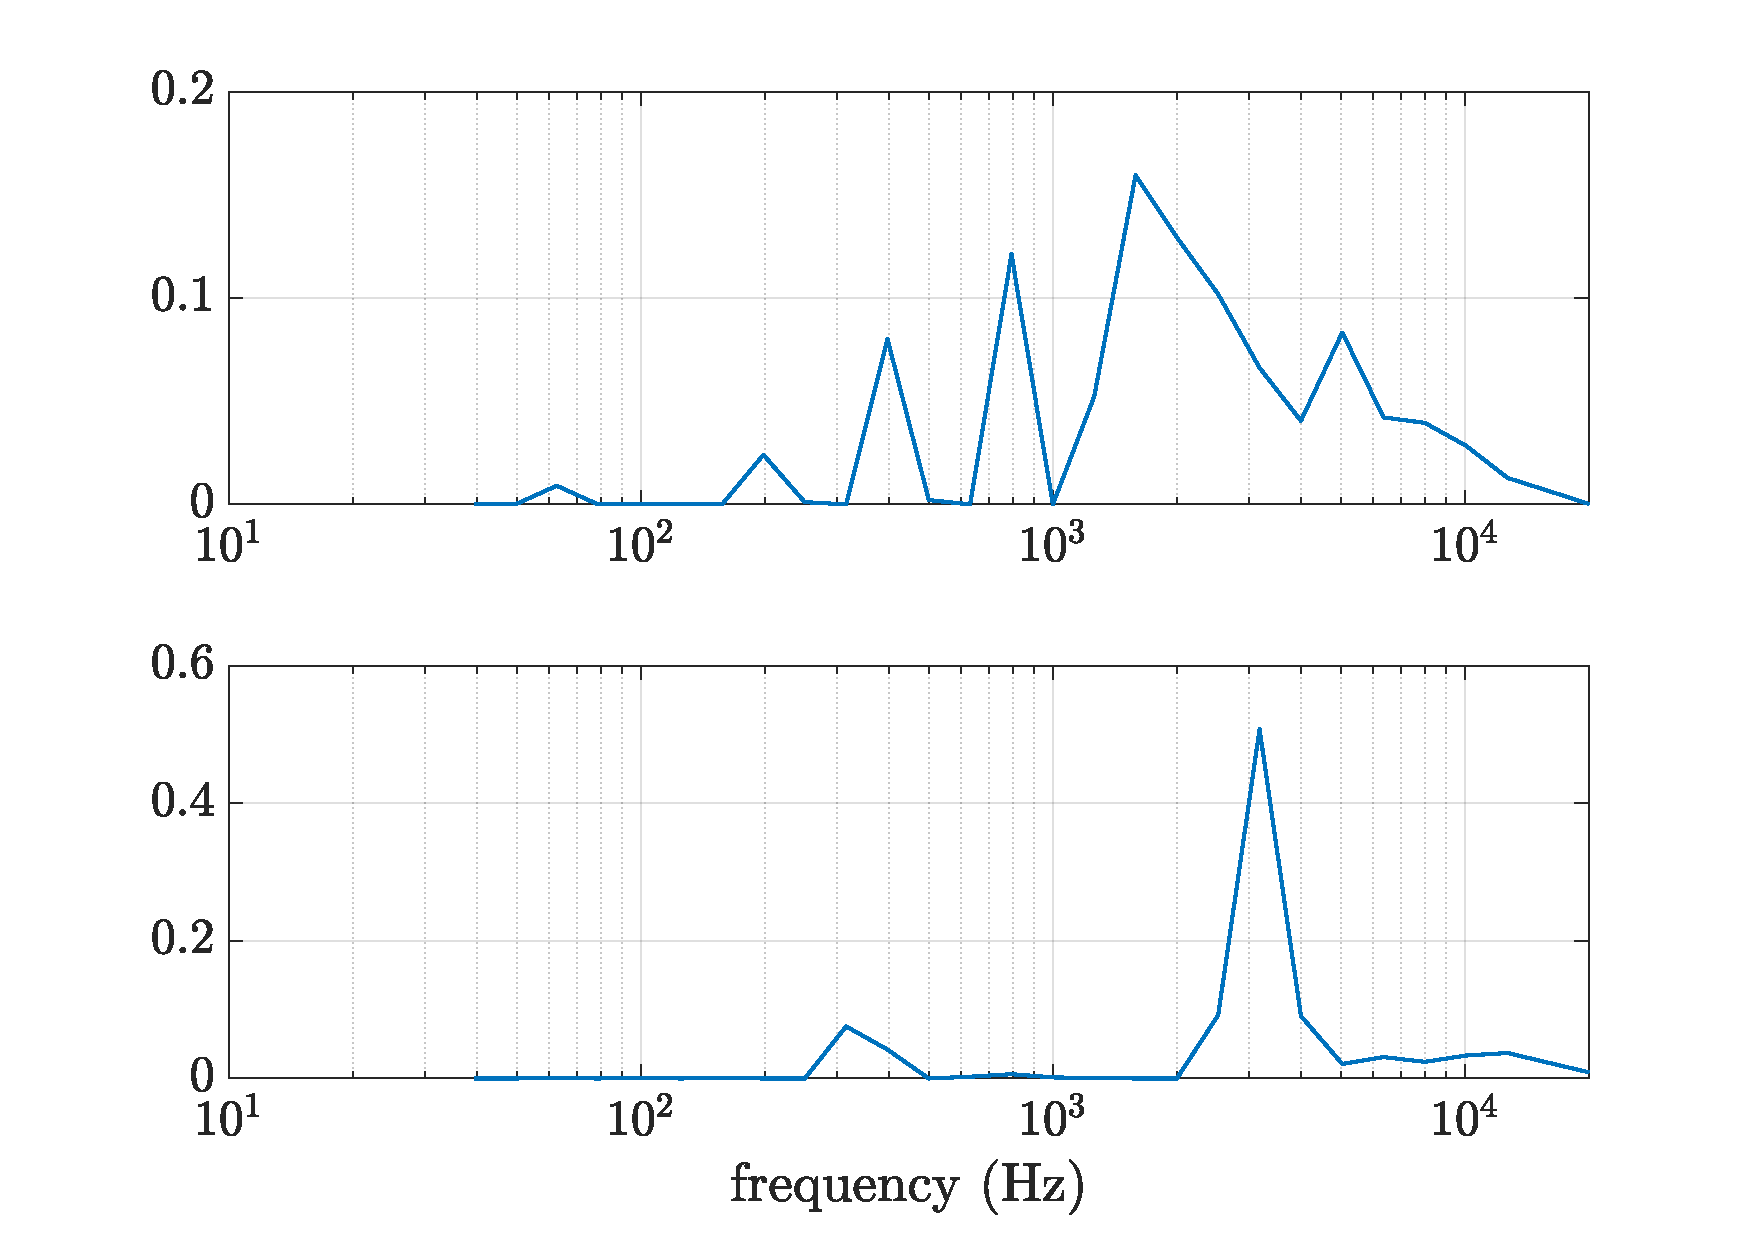
\includegraphics[width=\linewidth]{figures/Y_alert_-12.pdf}
        \caption{}
        \label{fig:Y_alert-12}
    \end{subfigure}%
    \hfill
    \begin{subfigure}[t]{0.45\textwidth}
        \centering
        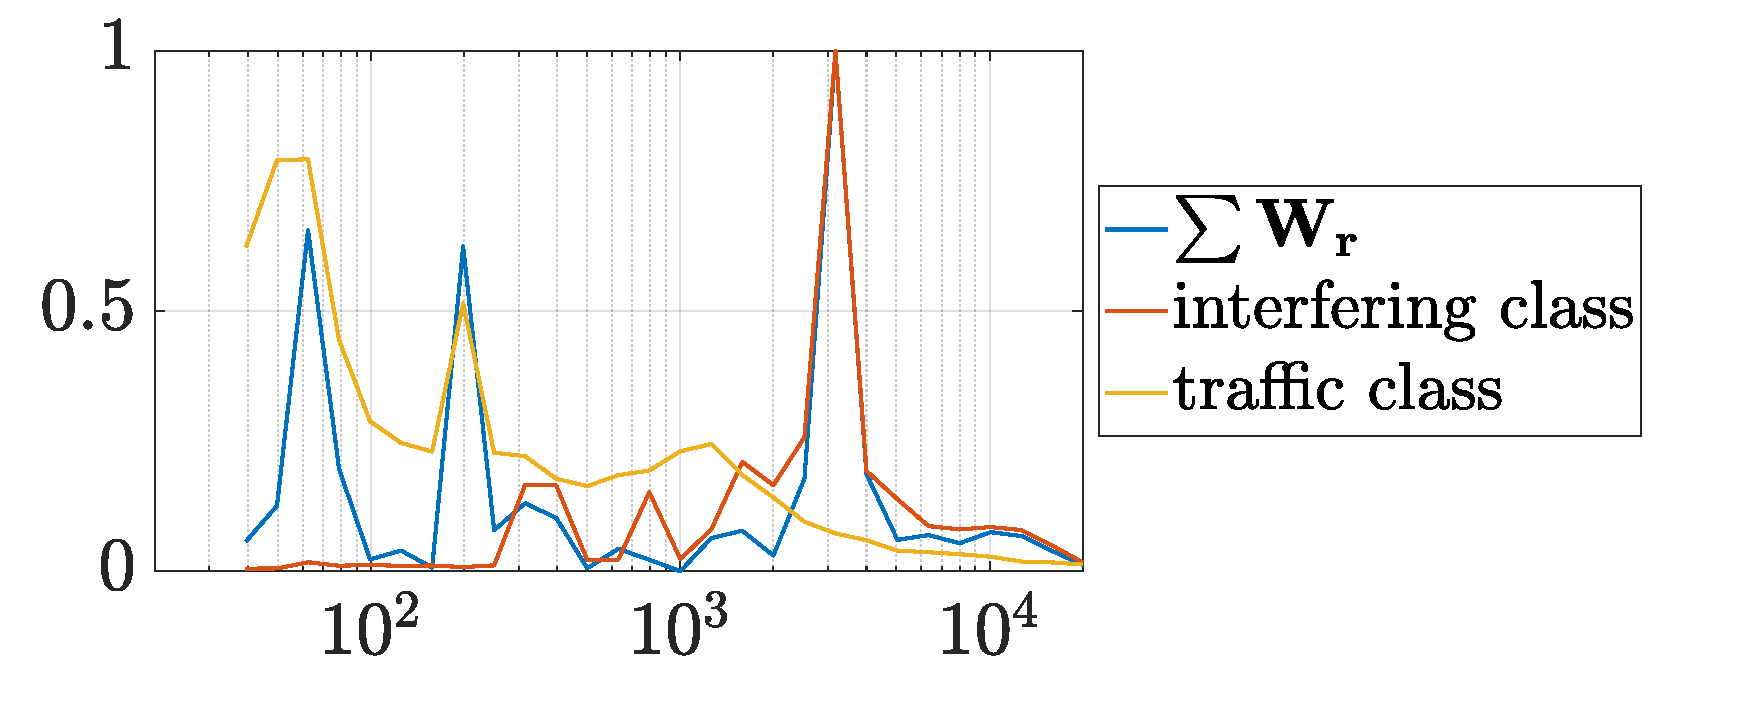
\includegraphics[width=\linewidth]{figures/Y_alert_12.pdf}
        \caption{}
		\label{fig:Y_alert_12}
    \end{subfigure}
    \caption{2 elements of $\mathbf{W_r}$ for an \textit{alert} scene for $TIR$ = -12 (\ref{fig:Y_alert-12}) and $TIR$ = 12 (\ref{fig:Y_alert_12})}
\end{figure*}


Finally, TI NMF with a threshold fixed at $t = 0.54$ and $\beta$ = 2, offers the lowest average results (Table \ref{tab:results}). If, according to each $TIR$, this method does not propose the lowest error, it succeeds to be a compromise between the two others NMF. Unlike SUP NMF, where $\mathbf{W}$ is fixed, and S-S NMF, where only $\mathbf{W_r}$ is updated, TI NMF updates $\mathbf{W}$ entirely to be adjusted to the scene and to adapt to the different sound environments. The closest elements of the \textit{traffic} component defined in $\mathbf{W_0}$ are then extracted to deduce the traffic signal. In Figure \ref{fig:dist_-12_12}, the similarity $D_{\theta}(\mathbf{W_0}||\mathbf{W})$ is displayed for 3 sub-classes for $TIR$ = [-12, 12] dB.

\begin{figure}[t]
    \centering
    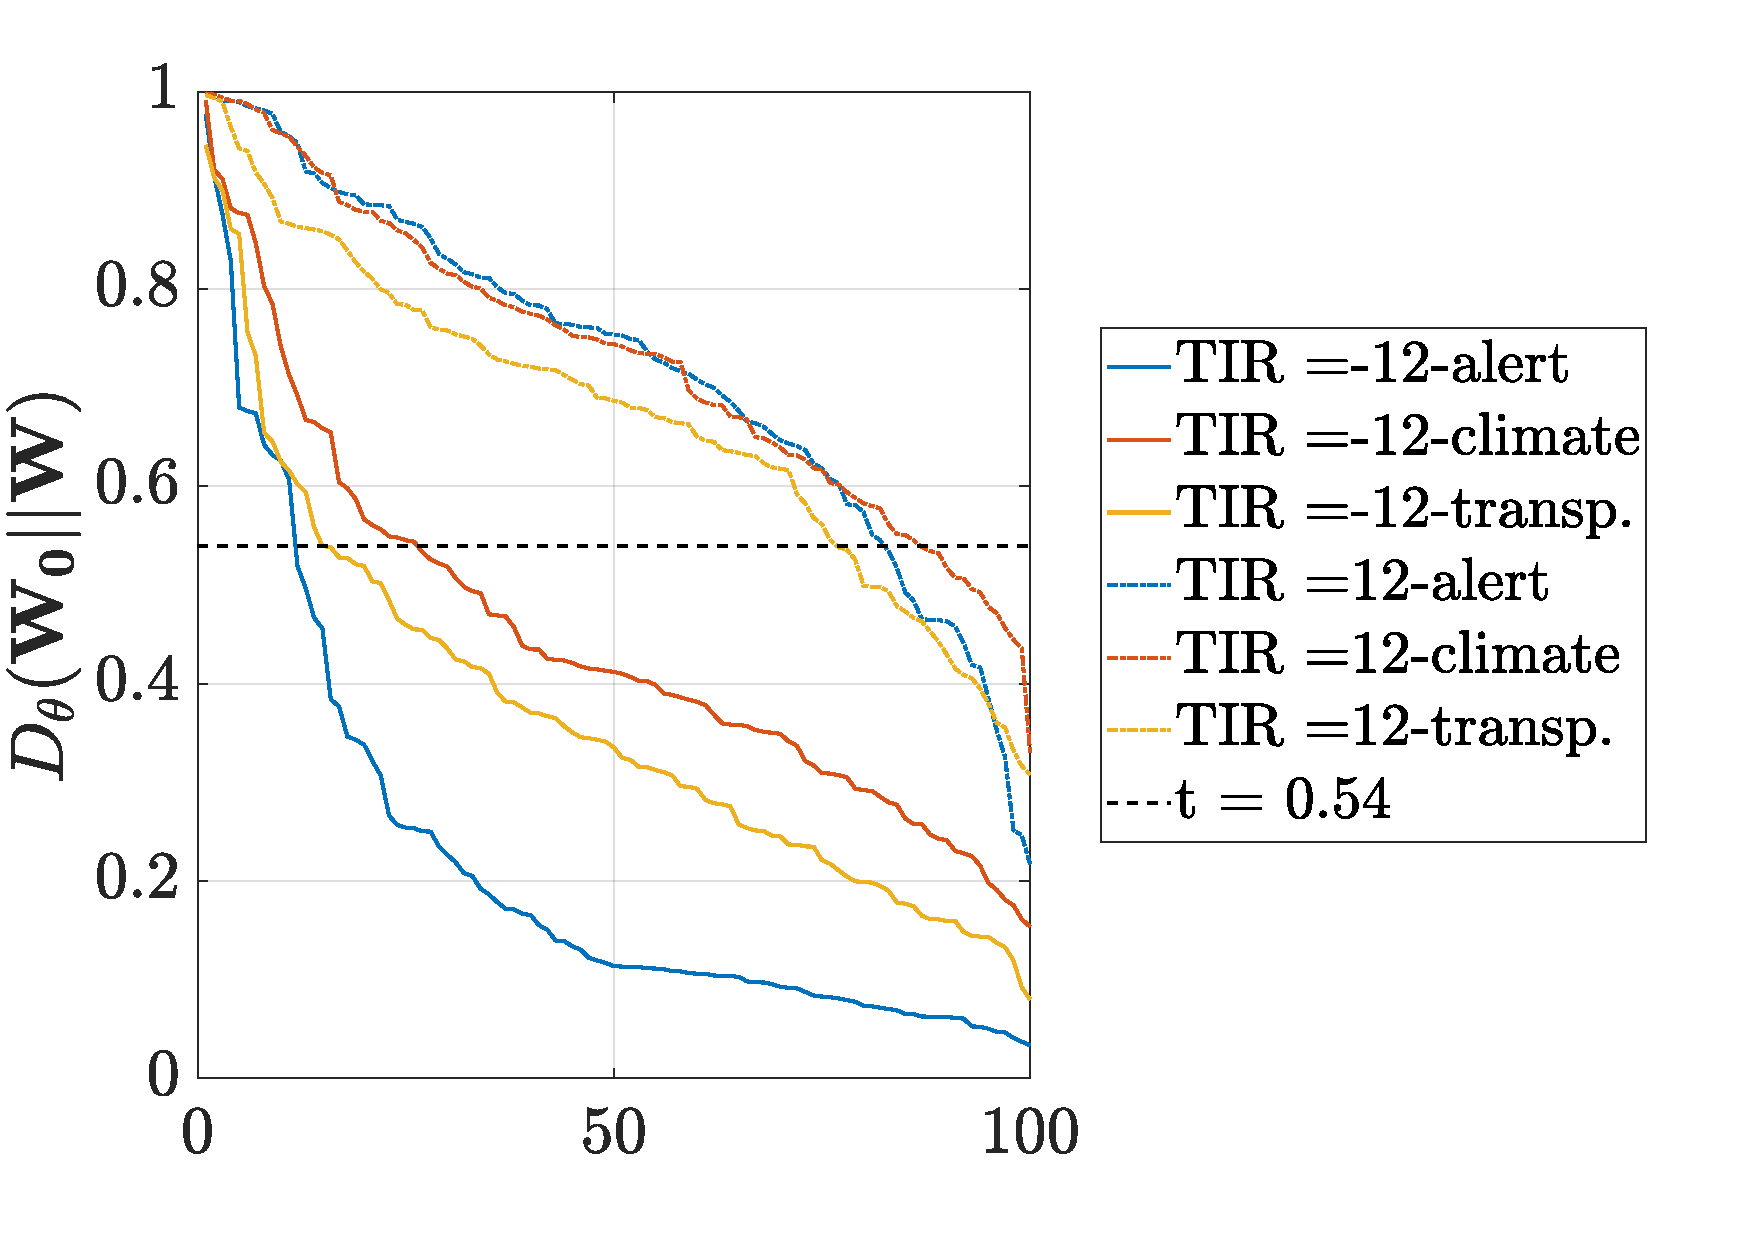
\includegraphics[width=\linewidth]{figures/dist_-12_12.pdf}
    \caption{Example of the similarity $D_{\theta}\left( \mathbf{W_0} \vert \vert \mathbf{W}\right)$ for different sub-classes and for two $TIR$ (-12 dB and 12 dB) and with the threshold $t$ = 0.54}
    \label{fig:dist_-12_12}
\end{figure}

For low $TIR$, as the traffic sound class is not predominant, the final dictionary differs a lot from the $\mathbf{W_0}$. With the thresholding, only a reduce number of basis vectors are considered as traffic components. In comparison to supervised results, this approach reduce significantly the error for the \textit{human} and \textit{transport} sub-classes.  However, for \textit{climate} and \textit{mechanics}, the error stay important as these interfering classes have similar spectrum. On high $TIR$, as the traffic is the main sound source, the similarity of the initial dictionary and $\mathbf{W}$ is higher which allows retaining more elements as traffic components and then decrease the error (< 1 dB). The kept elements are then more suited to the scenes than a fixed dictionary. The error for these $TIR$ is then due to the thresholding. With a low threshold, it is possible to decrease the error (for $TIR$ = 12 dB, the average error on all the sub-classes is 0.22 ($\pm$ 0.08) dB with $t$ = 0.30).

\section{Conclusion}

In this work, NMF, a source separation method, was used to estimate the road traffic sound level in urban sound mixtures. It is an adapted approach to these sound environments because it easily takes into account the overlap between the multiple sound sources present in the cities and is adapted to monophonic sensor networks. Different versions of NMF have been studied as a supervised and semi-supervised approach. On a large corpus of sound, the supervised approach proves to be too restrictive to be adapted to different sound environments whereas the semi-supervised approach has, on the contrary, too many degrees of freedom on the mobile dictionary $\mathbf{W_r}$, decreasing its performance especially when the traffic is predominant. The proposed new approach, named Threshold Initialized NMF, where $\mathbf{W}$ is initialized with road traffic spectrum, updated and where the traffic elements are extracted by hard thresholding, proposes the lowest average error. It allows a compromise between the other two approaches where a prior knowledge of the targeted sound source is given as in the SUP NMF, and offers an adaptability to the different sound mixtures by updating $ \mathbf{W}$ entirely.

This method has the advantage to keep a low calculation cost and then can be implemented in embedded sensors. Furthermore, this approach stay adapted for other sound sources, as whistling bird, depending on what spectrum are put in $\mathbf{W}$ and can be adapted for other application than the road traffic sound level estimation. Finally, the add of constraints as sparsness \cite{hoyer2004non} and smoothness \cite{virtanen_monaural_2007} can easily be implemented and taken into account.

In parallel, this experience allowed the design of a large sound database composed of multiples samples of urban sounds and sound mixtures that are made available\footnote{\url{https://sandbox.zenodo.org/record/176695#.Wk4ow3kiGos}} for research communities dedicated to the detection, separation and recognition tasks of urban sound sources.
The experience has been lead with the Matlab software. In order to be a reproducible experience, all the programs\footnote{\url{https://github.com/jean-remyGloaguen/article2017EstimationAmbiance}} used for this experience are available online.

\footnotesize
\bibliographystyle{unsrt}
\bibliography{bibliographie_applied}

\end{document}
